This chapter discusses the transient multiphysics simulation results of the
\gls{MSFR} from Moltres for four accident scenarios. These scenarios, adapted
from Fiorina et al.'s work \cite{fiorina_modelling_2014}, include unprotected
instances of reactivity insertion, loss of heat sink, loss of flow, and pump
overspeed accidents. The term ``unprotected'' means that there is no
external intervention in these scenarios. As such, these simulations
give an insight on the \gls{MSFR}'s passive safety capabilities in the absence
of any active safety system. We used the steady-state configuration presented
in the previous chapter as the initial conditions for the transient
simulations discussed in this chapter. Specifically, we imported all
steady-state spatial values for neutron flux, delayed neutron precursor
concentration, temperature, velocity, and pressure as the initial state of the
transient scenarios.

As noted by Fiorina et al. \cite{fiorina_modelling_2014}, explicit decay heat
modeling has a negligible effect in reactivity-, and pump-initiated
transients. Furthermore, only their Polimi model had decay
heat modeling capabilities. Therefore, they presented results from their
Polimi and TUDelft model for the four accident scenarios  without decay heat
modeling; they enabled decay heat modeling for the loss of heat sink transient
scenario only. For a direct comparison, we also ran all transient simulations
without the decay heat model with the exception of the loss of heat sink
scenario in which we ran two separate simulations with and without
the decay heat model. More generally, we imposed various other simplifying
assumptions in our transient models to match their implementations as closely
as possible, within Moltres' capabilities. The details of the setup for each
transient simulation are in their respective sections.

\section{Unprotected Reactivity Insertion}

\glspl{RIA} are a type of nuclear accident caused by unintended positive
reactivity insertions. The excess reactivity causes the power output and
temperatures in nuclear reactors to rise to potentially dangerous levels. In
\glspl{MSR}, a positive reactivity insertion could occur when the online
refueling system injects excess fissile material into the core. Excessively
high neutron fluences and temperatures negatively impact reactor structural
integrity and increase the risk of containment breach.

We modeled two unprotected step-wise reactivity insertion scenarios in Moltres
by swapping out the original set of group constant data with two new, separate
sets of data from Serpent corresponding to 50 pcm and 200 pcm reactivity
insertions, respectively. We increased the reactivity of the Serpent
\gls{MSFR} models by increasing the $^{233}$U-to-$^{232}$Th ratio in the fuel
salt.

The focus of this transient study is the neutronic and thermal-hydraulic
behavior of the reactor core. Thus, we assume that the heat exchanger and the
associated power generation equipment (generator turbines, heat sinks, etc.)
can withstand all variations in the power output during the transients.

Figures \ref{fig:50pcmheat} and \ref{fig:50pcmtemp} show the power output and
average core temperature increase following the 50 pcm step-wise reactivity
insertion in the Moltres, Polimi, and TUDelft models. The initial prompt
response to the reactivity insertion raises power to 4 GW by $t=0.001$ s.
Figure \ref{fig:50pcmjump} shows the rise in power output specifically during
the prompt response in a separate plot.
Power continues to rise at a slower rate up to 4.63 GW at around $t=0.005$ s,
at which point the negative reactivity from the Doppler effect and salt
expansion becomes greater
than the initial +50 pcm insertion. Power continues to fall as the average
core temperature rises. There is a slight change in slope at $t=0.3$ s. This
value approximately corresponds to the average half-life of the two
shortest-lived delayed neutron precursor (DNP) groups ($t_{1/2}=0.195$ s and
$0.424$ s); the decay of the surplus precursors produced in the initial phase
negates a fraction of the negative reactivity from the elevated core
temperature. By $t=3$-$4$ s, most of the heated salt and \glspl{DNP} from the
initial phase will have circulated around the primary loop and returned to the
core. The heated salt causes a small, noticeable dip in power before the power
output stabilises. The core tends to a new equilibrium average temperature
approximately 7.5 K higher than the initial average temperature.

\begin{figure}[htbp!]
    \centering
    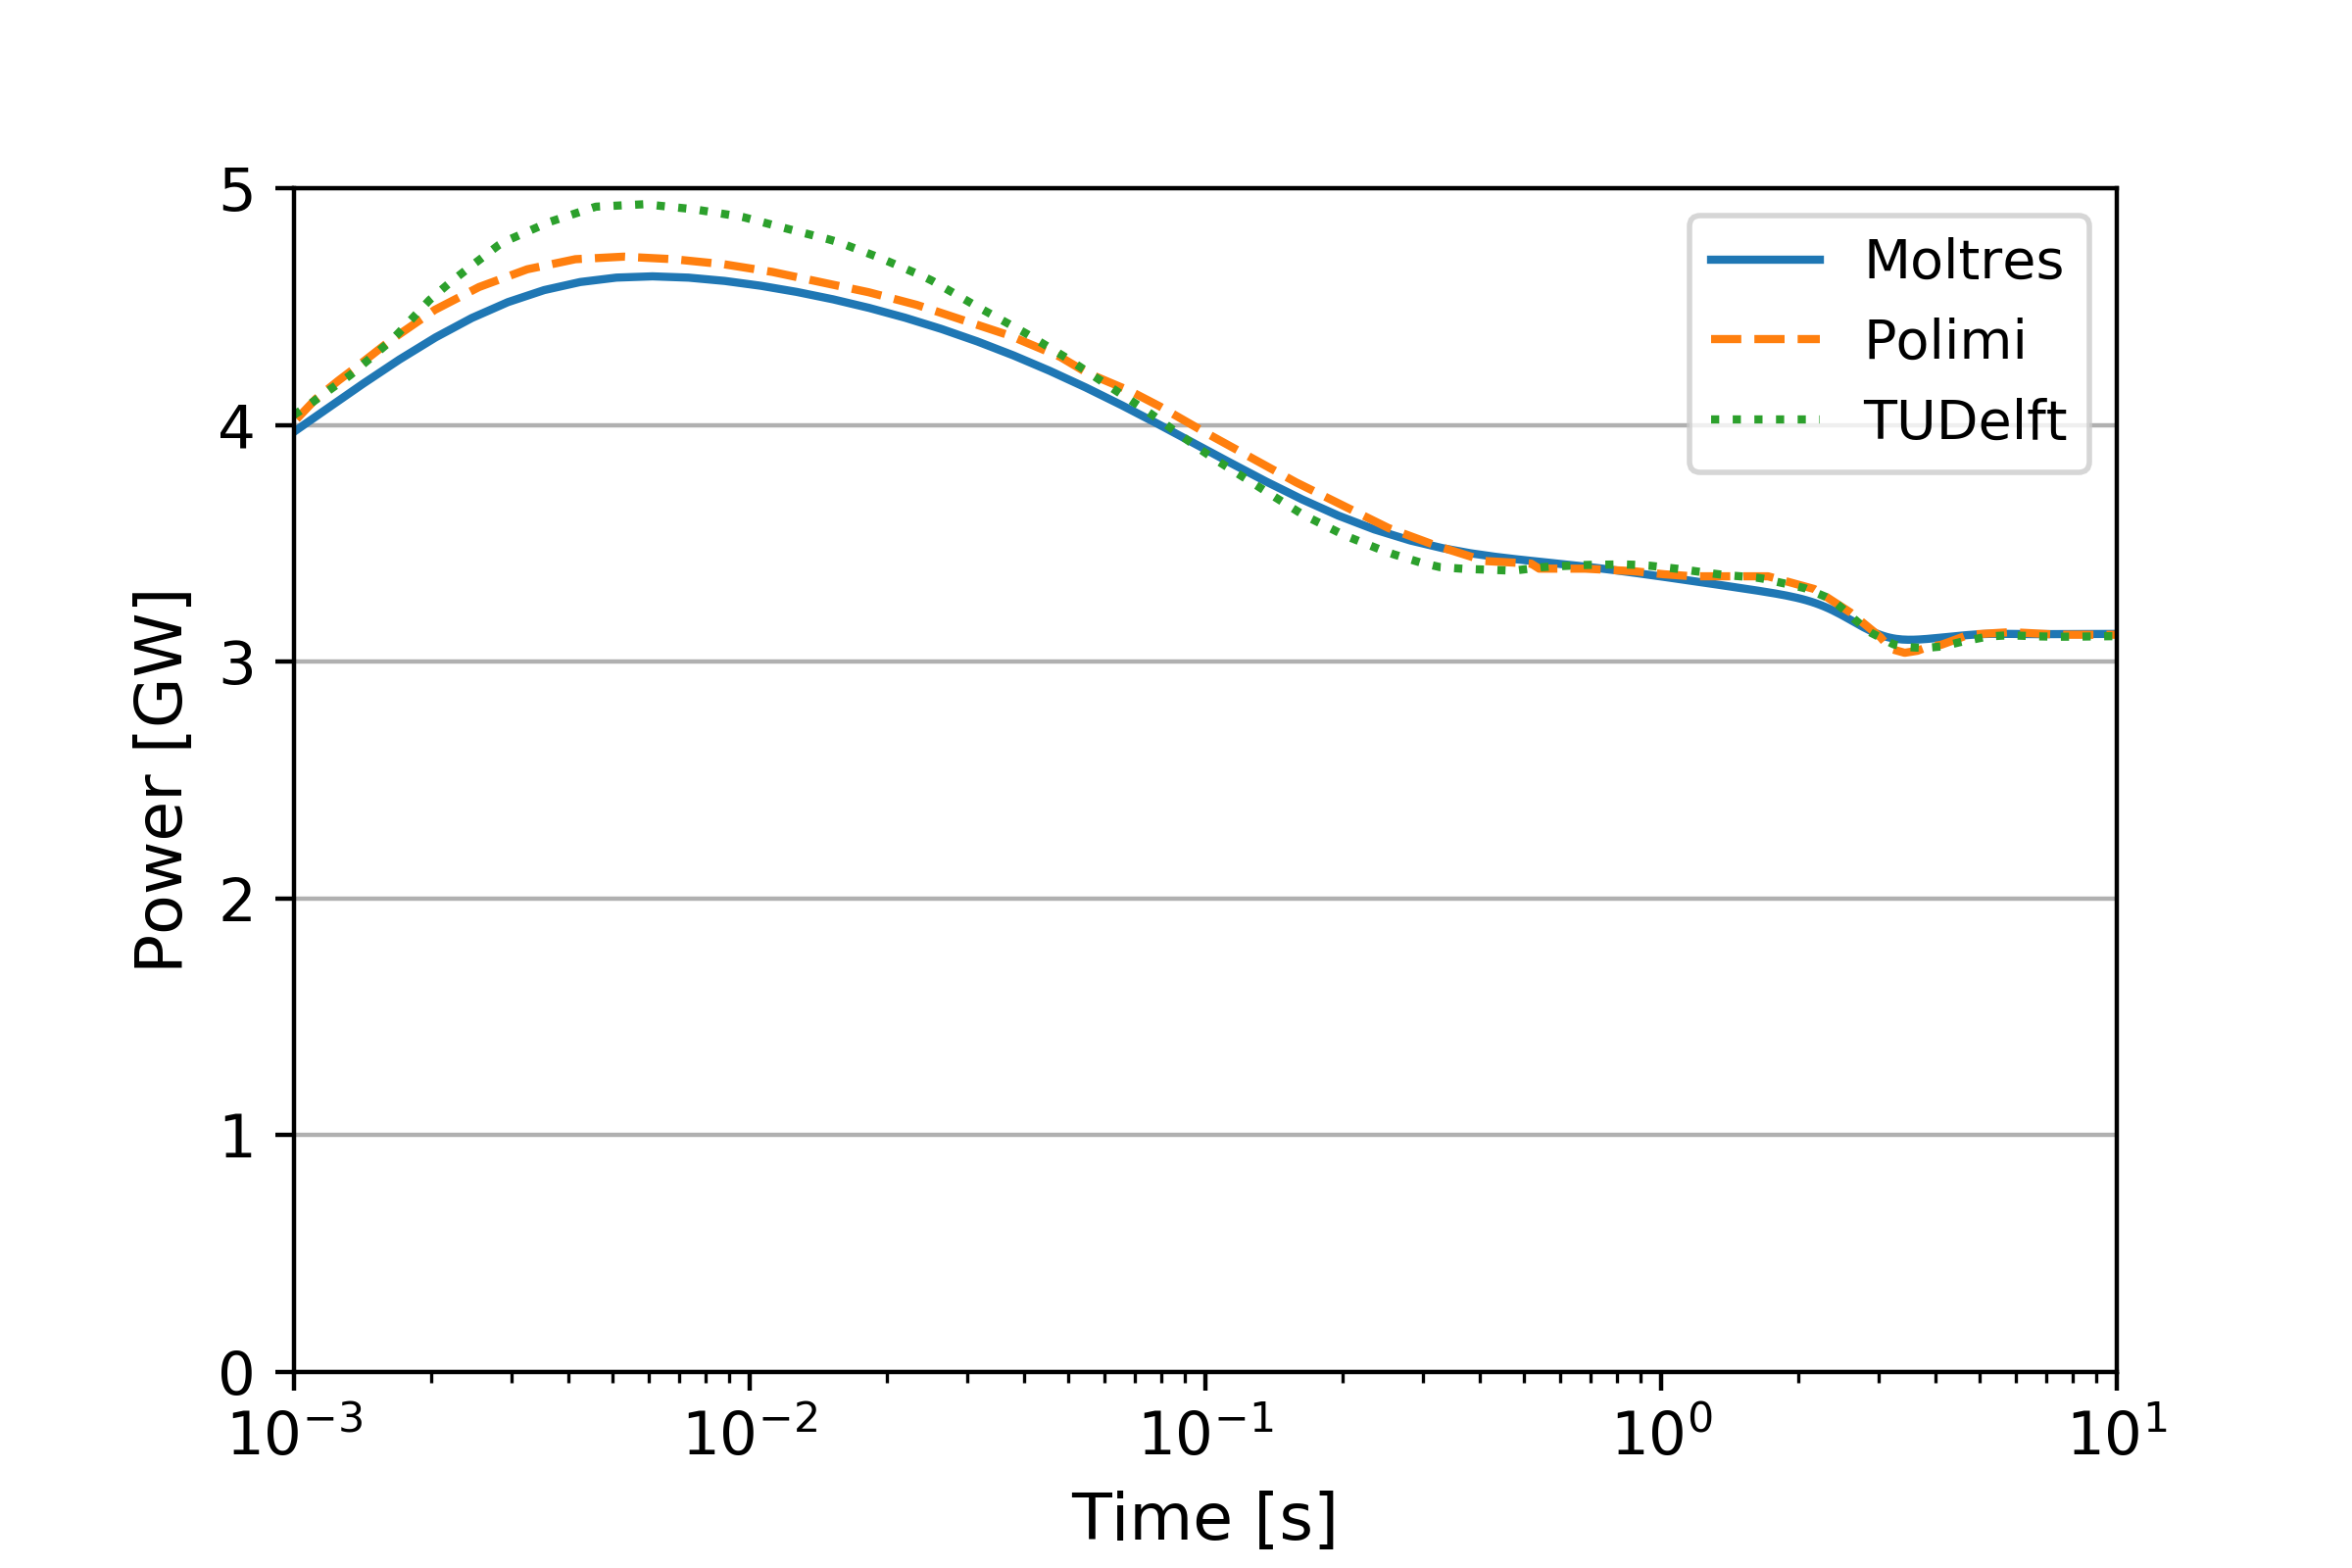
\includegraphics[width=.85\textwidth]{50pcm-heat}
    \caption{Power output following
    a 50 pcm step-wise reactivity insertion in the Moltres, Polimi, and
    TUDelft models \cite{fiorina_modelling_2014}.}
    \label{fig:50pcmheat}
%
    \centering
    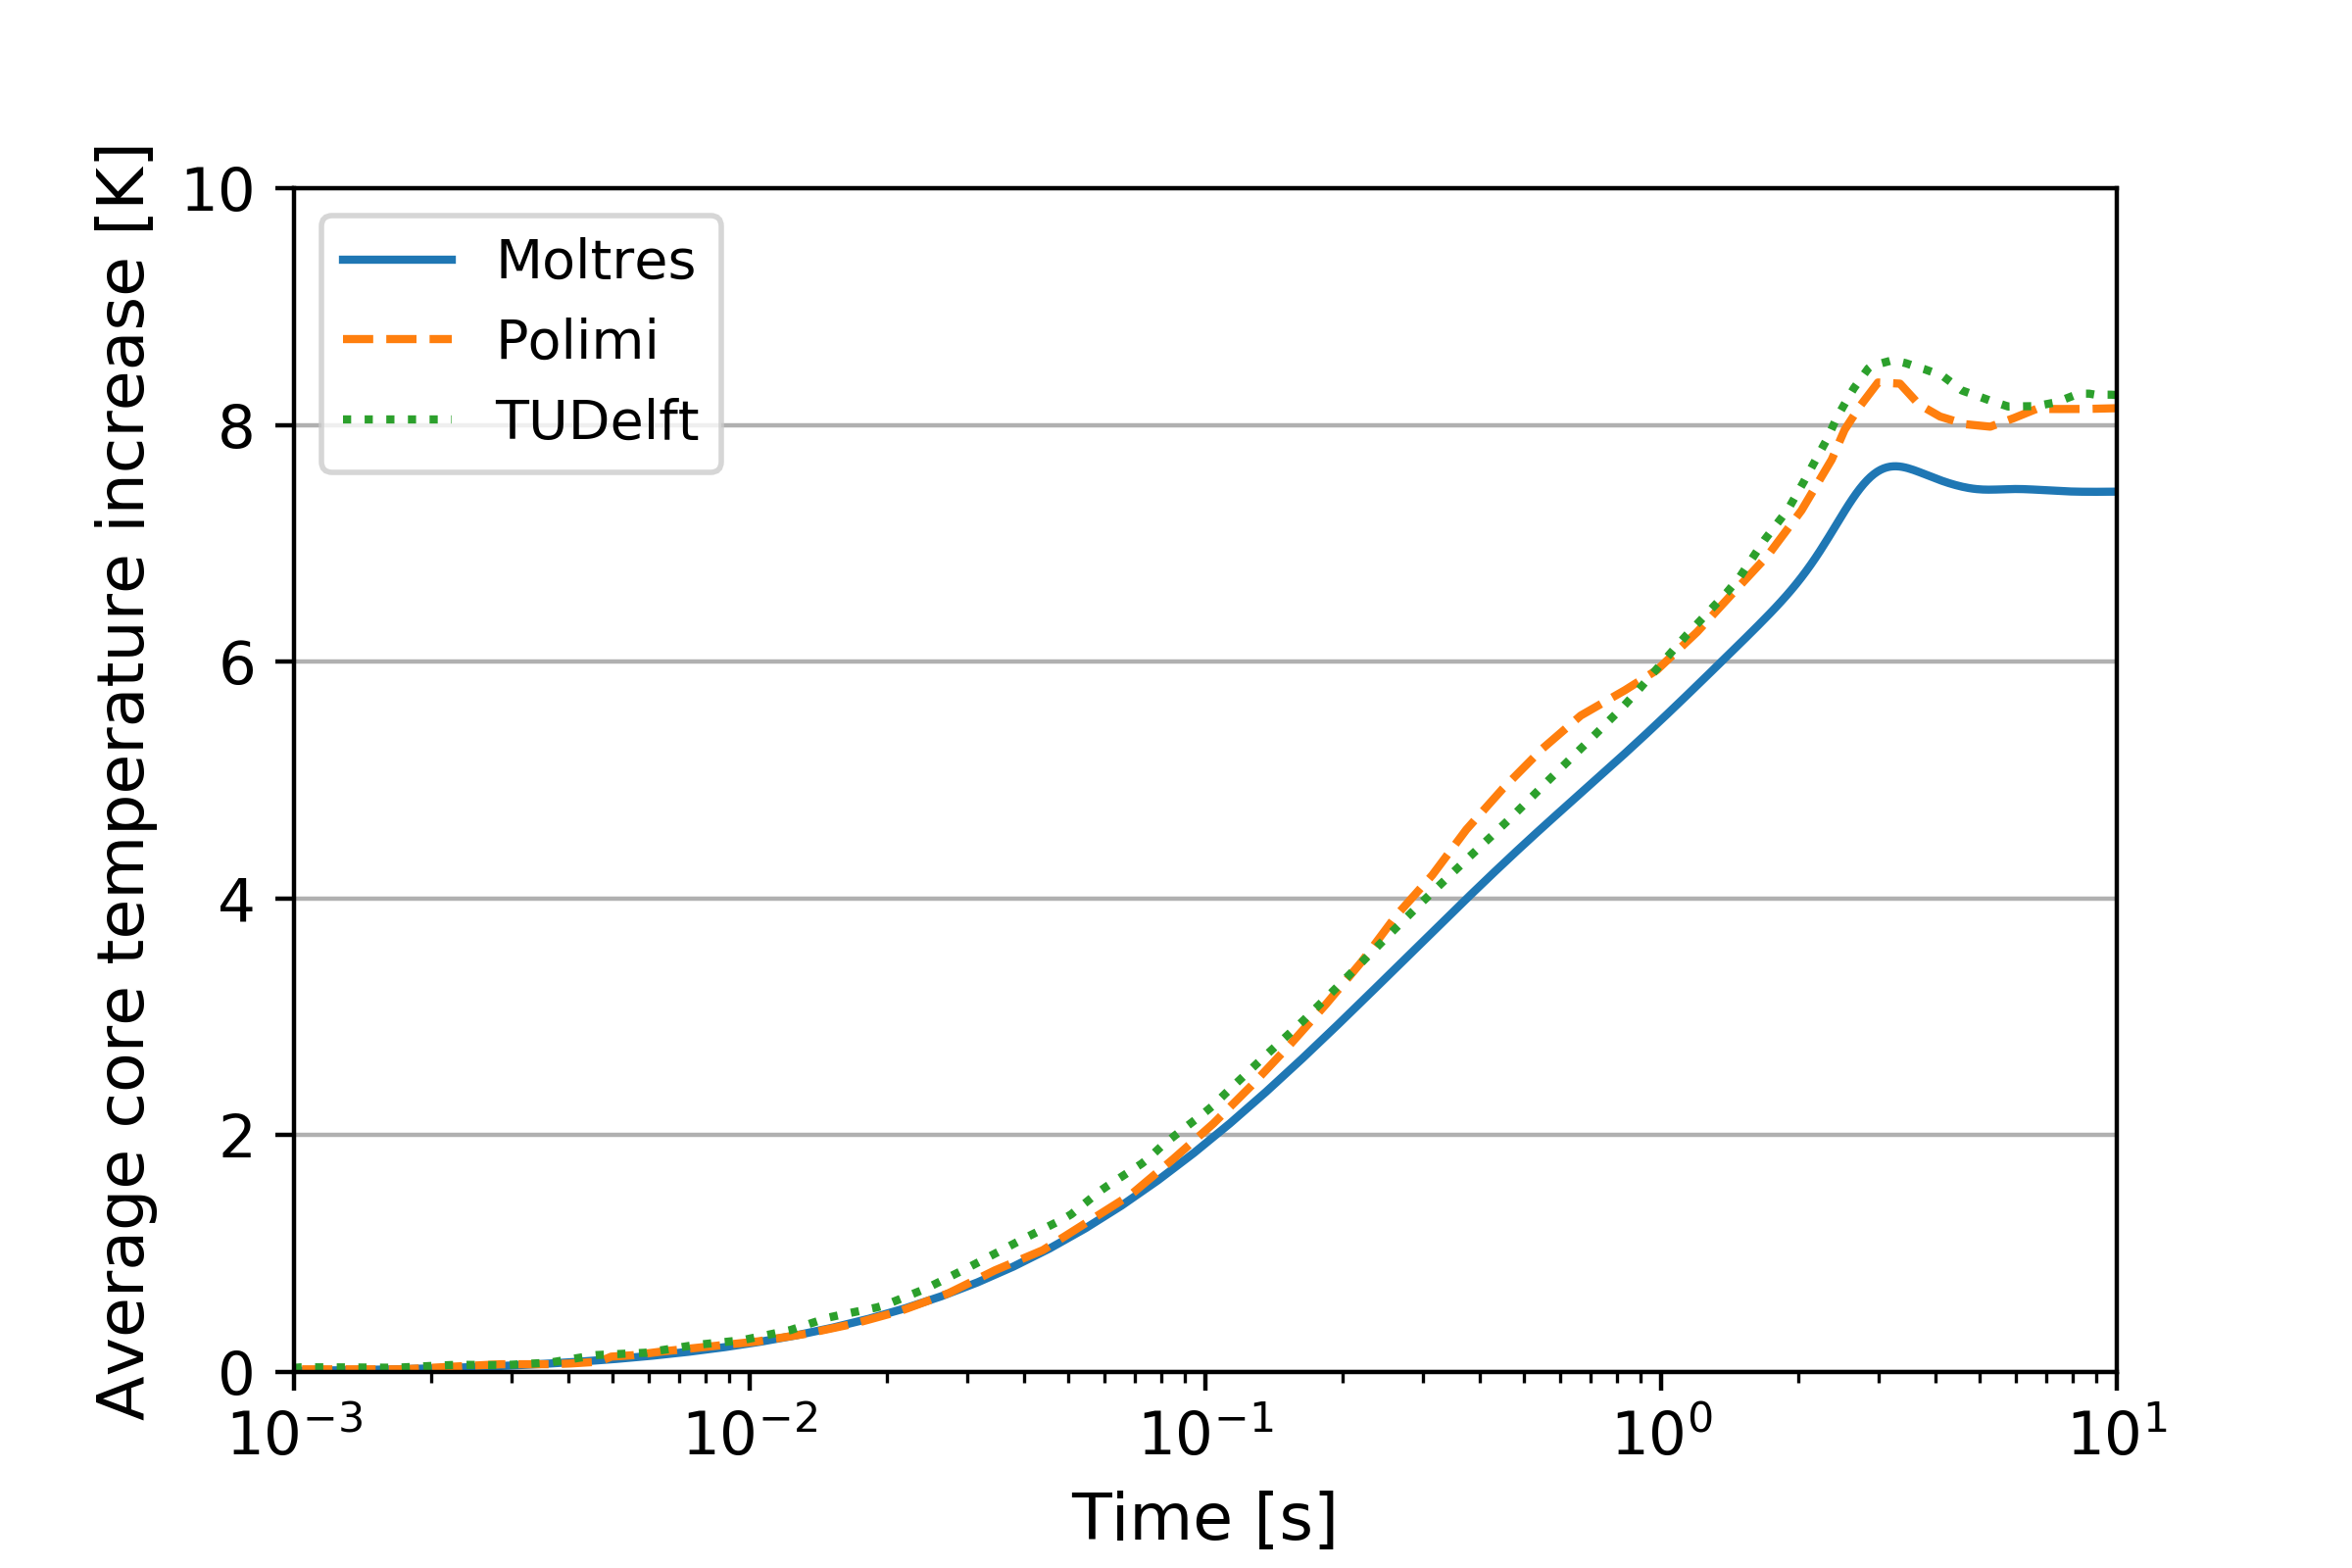
\includegraphics[width=.85\textwidth]{50pcm-temp}
    \caption{Average core temperature increase following
    a 50 pcm step-wise reactivity insertion in the Moltres, Polimi, and
    TUDelft models \cite{fiorina_modelling_2014}.}
    \label{fig:50pcmtemp}
\end{figure}

\begin{figure}[htbp!]
    \centering
    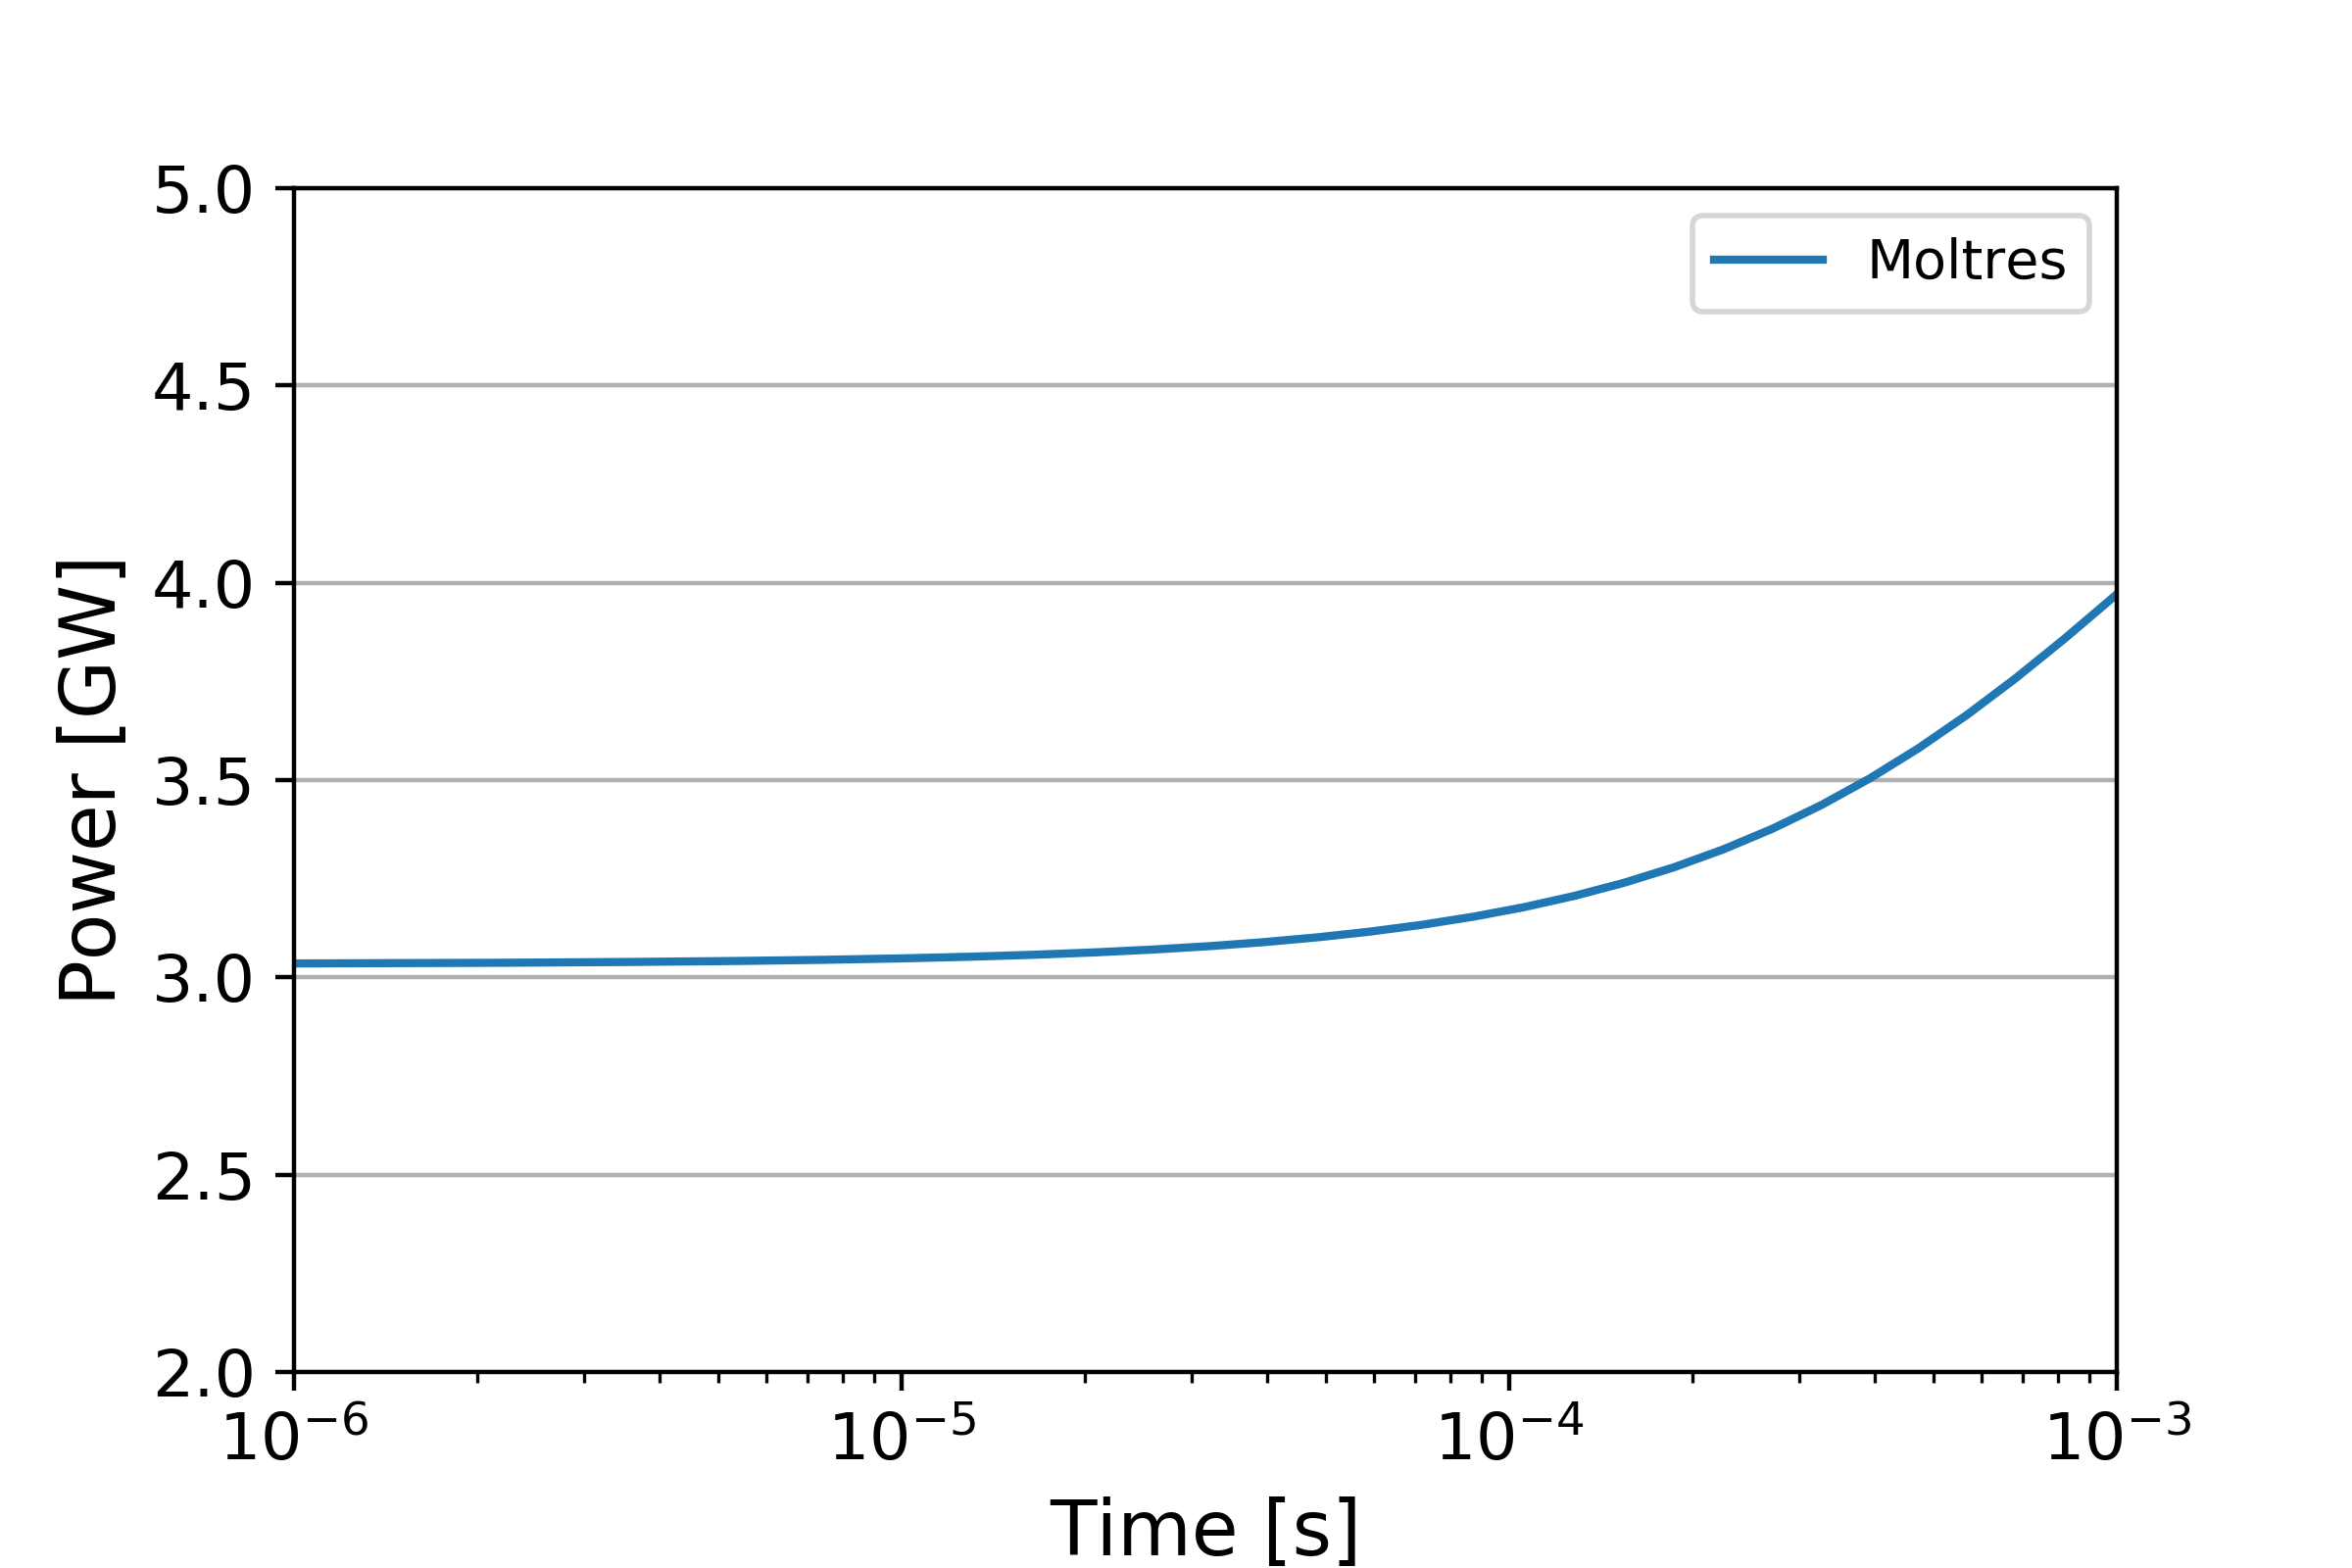
\includegraphics[width=.7\textwidth]{50pcm-jump}
    \caption{Power output during the prompt response following
    a 50 pcm step-wise reactivity insertion in the Moltres, Polimi, and
    TUDelft models \cite{fiorina_modelling_2014}.}
    \label{fig:50pcmjump}
\end{figure}

The results from Moltres show good agreement with the results from the Polimi
and TUDelft models; Moltres reproduced all of the individual features in both
plots. The most significant difference is in the magnitude of the reactor
response. Moltres predicts a smaller peak in the power output and a smaller
overall increase in the average core temperature. This is largely due to the
more negative temperature reactivity coefficient in Moltres than in the Polimi
and TUDelft models. The temperature reactivity coefficient $\alpha_T$ in
Moltres is $-7.184$ pcm K$^{-1}$ (Table \ref{table:alpha}), as opposed to
approximately $-6.5$ pcm K$^{-1}$ within the relevant temperature range in the
Polimi and TUDelft models. Therefore, we see a smaller temperature increase in
the Moltres model for the same reactivity insertion. Multiplying the average
core temperature increase at $t=10$ s with $\alpha_T$ gives us $-7.184$ pcm
K$^{-1} \times 7.46$ K $= -53.6$ pcm, which is approximately equal to the 50
pcm reactivity insertion.

\begin{figure}[htbp!]
    \centering
    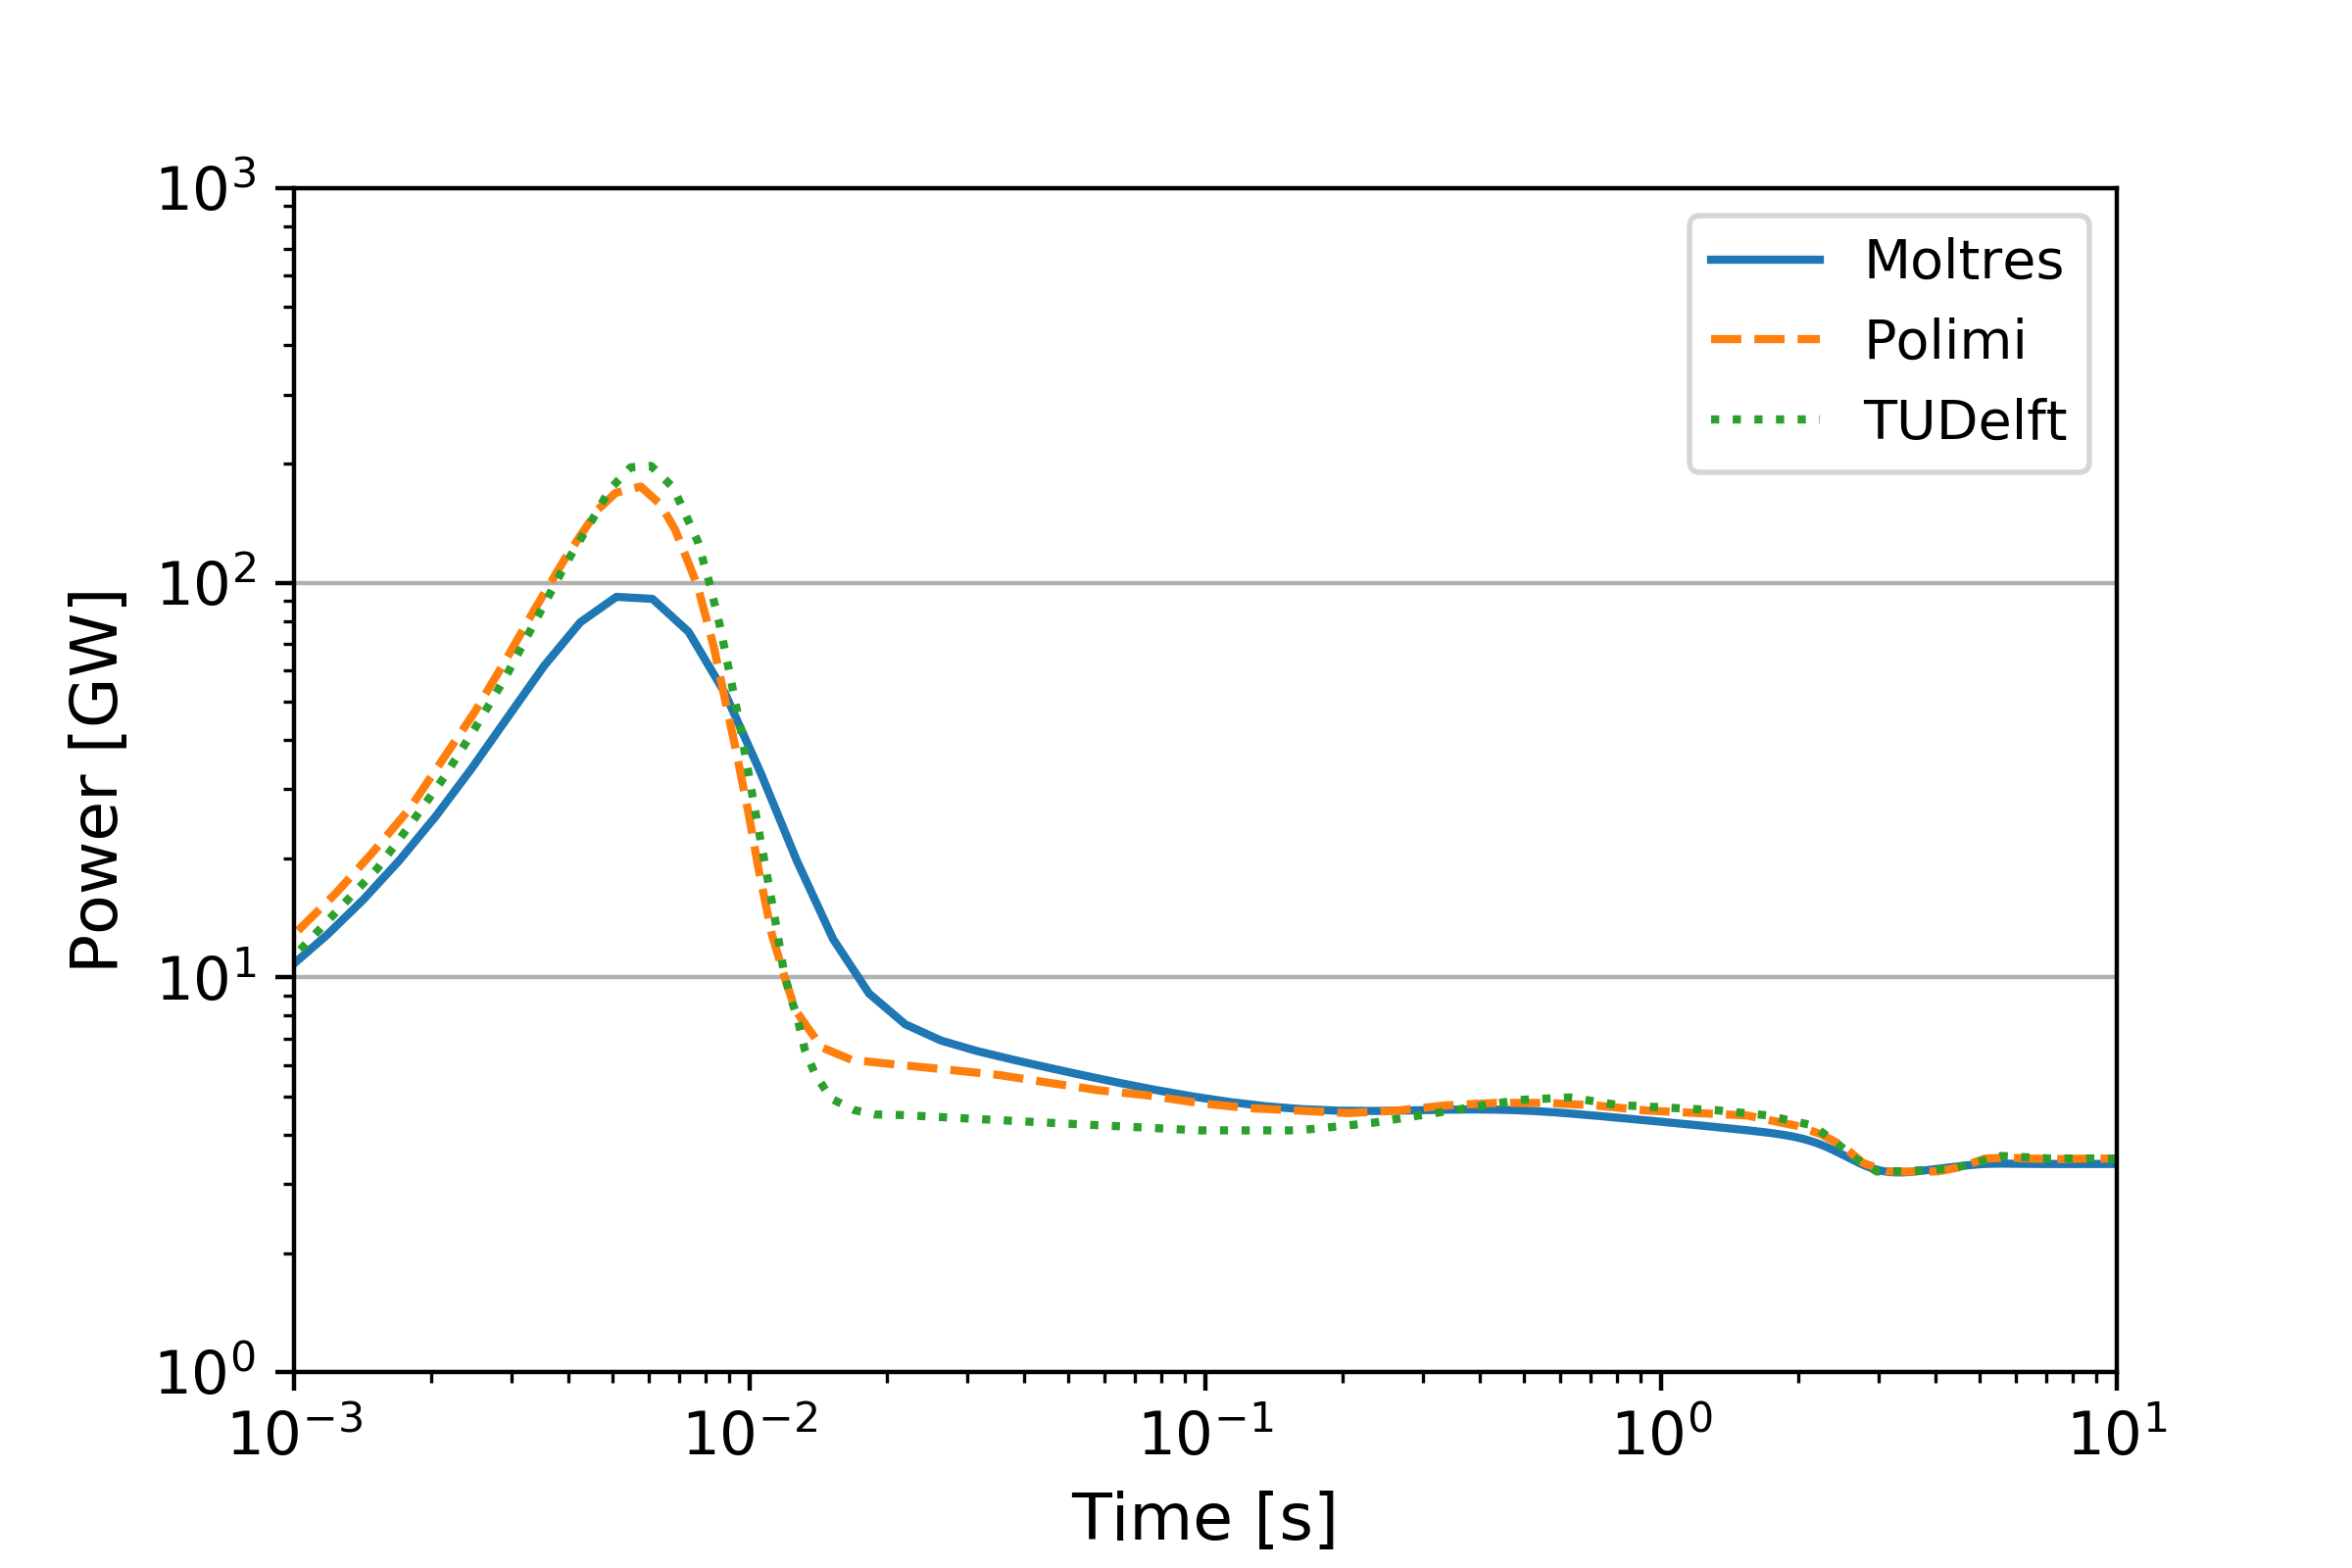
\includegraphics[width=.85\textwidth]{200pcm-heat}
    \caption{Power output following
    a 200 pcm step-wise reactivity insertion in the Moltres, Polimi, and
    TUDelft models \cite{fiorina_modelling_2014}.}
    \label{fig:200pcmheat}
%
    \centering
    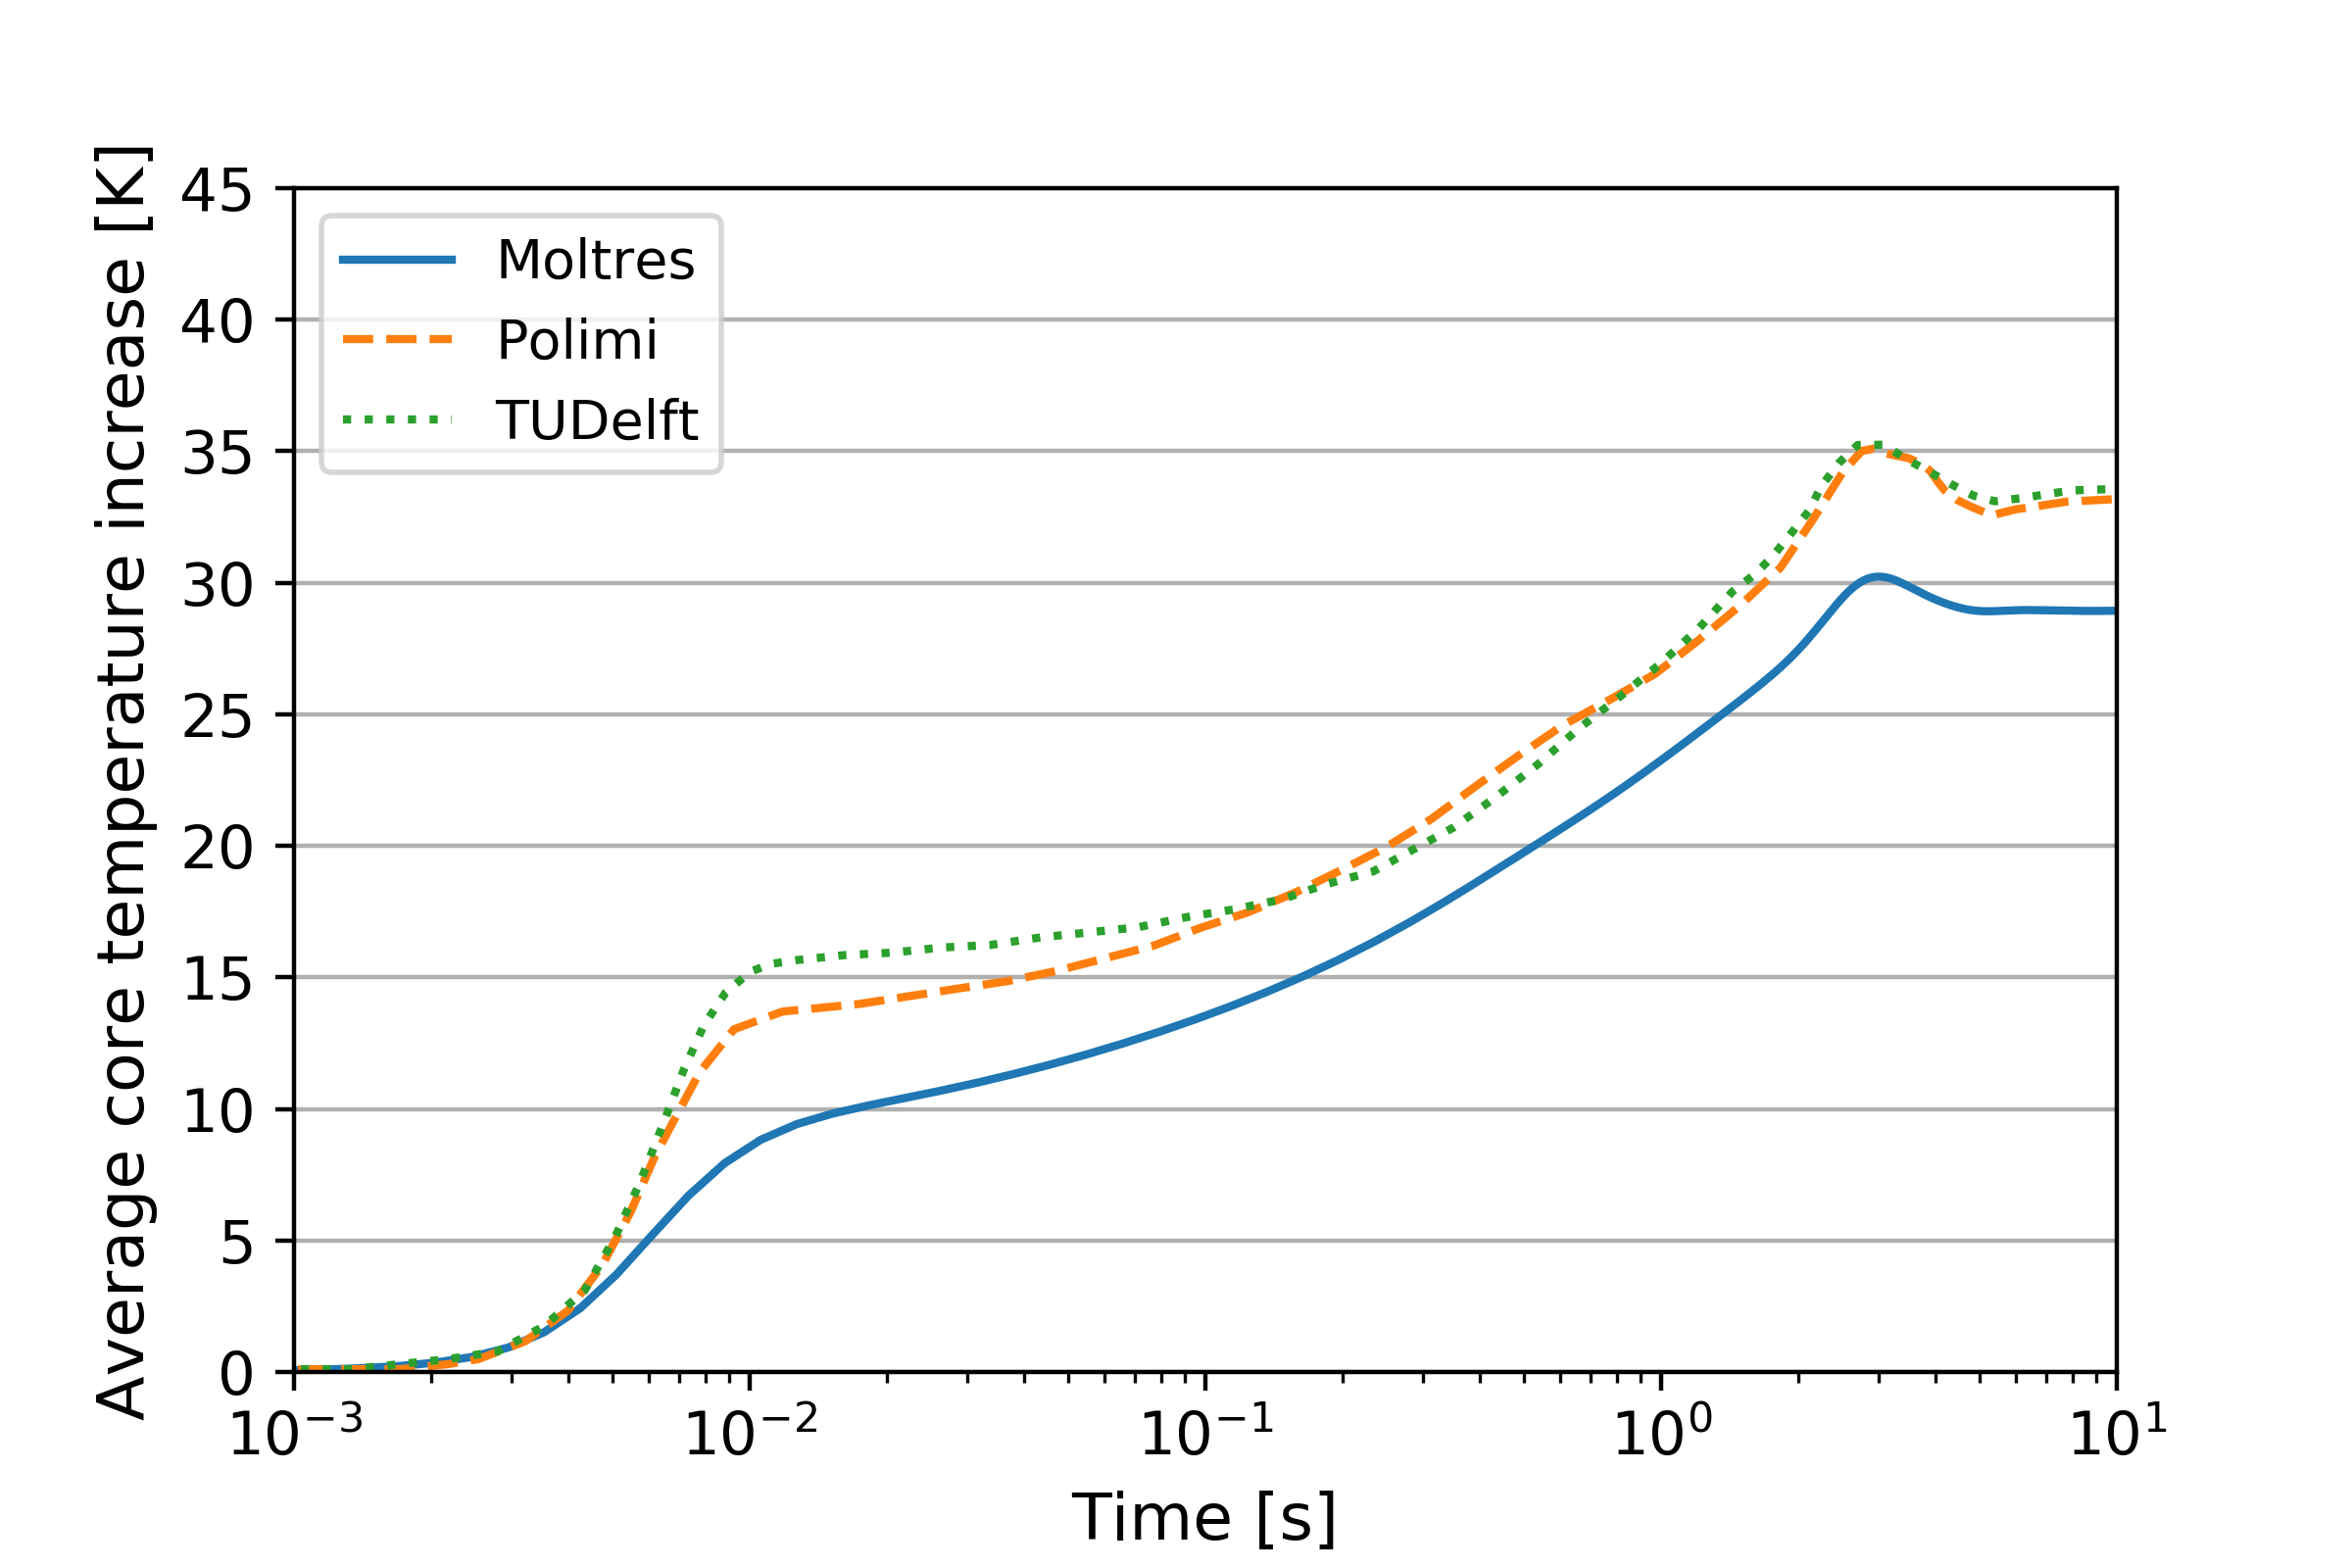
\includegraphics[width=.85\textwidth]{200pcm-temp}
    \caption{Average core temperature increase following
    a 200 pcm step-wise reactivity insertion in the Moltres, Polimi, and
    TUDelft models \cite{fiorina_modelling_2014}.}
    \label{fig:200pcmtemp}
\end{figure}

The results for the 200 pcm reactivity insertion scenario show similar trends
to the 50 pcm case. The larger reactivity insertion illicits a stronger
prompt response in the power output which peaks at 92.1 GW. The average core
temperature increases much more rapidly and subsequently triggers a sharper drop in power output. This results in the clearer distinction in the rate of
core temperature increase before and after $t=0.01$ s. In this transient, we
also observe greater deviation between Moltres and the other models arising
from the differences in the temperature reactivity coefficients. Overall,
Moltres' results show good agreement with the Polimi and TUDelft results and
the differences arise mainly due to the differences in the temperature
reactivity coefficients.

\clearpage

\section{Unprotected Loss of Heat Sink}

An unprotected loss of heat sink accident can occur when the pumps in the
intermediate loop fail. The heat exchangers would then lose most of their
cooling capabilities. We followed Fiorina et al.'s approach in assuming that
the cooling from the heat exchangers decreases exponentially with a time
constant of 1 s and all other parameters held constant
\cite{fiorina_modelling_2014}. As mentioned in the Chapter \ref{chap:ss}, we
will present two sets of results for this transient: 1) without decay heat modeling, and 2) with decay heat modeling.

\subsection{Without Decay Heat}

Figures \ref{fig:lohsheat} and \ref{fig:lohstemp} show the power output and
average core temperature increase during the unprotected loss of heat sink
transient in the Moltres, Polimi, and TUDelft models without decay heat
modeling. The power output and average core temperature show little change in
the first two seconds as it takes approximately that amount of time for the
partially cooled salt to migrate to the center of the core. At $t=2$ s, we
observe a sharp spike in average core temperature and a corresponding drop
in power output. The presence of delayed neutron precursors (DNPs) from the
steady-state operating conditions momentarily halt the increase in temperature
at around $t=5$ s. The average core temperature continues to rise while the
power output falls through the rest of the transient.

The results from Moltres show good agreement with the results from the Polimi
and TUDelft. Moltres reproduced all of the trends that we see in the Polimi
and TUDelft models. The temporary halt in the temperature increase occurs at
a lower average core temperature for Moltres than the other two models. This
is likely due to the difference in the temperature reactivity coefficient
that we discussed in the reactivity insertion results; a smaller increase in
the average core temperature produces the same decrease in power output.

\begin{figure}[htbp!]
    \centering
    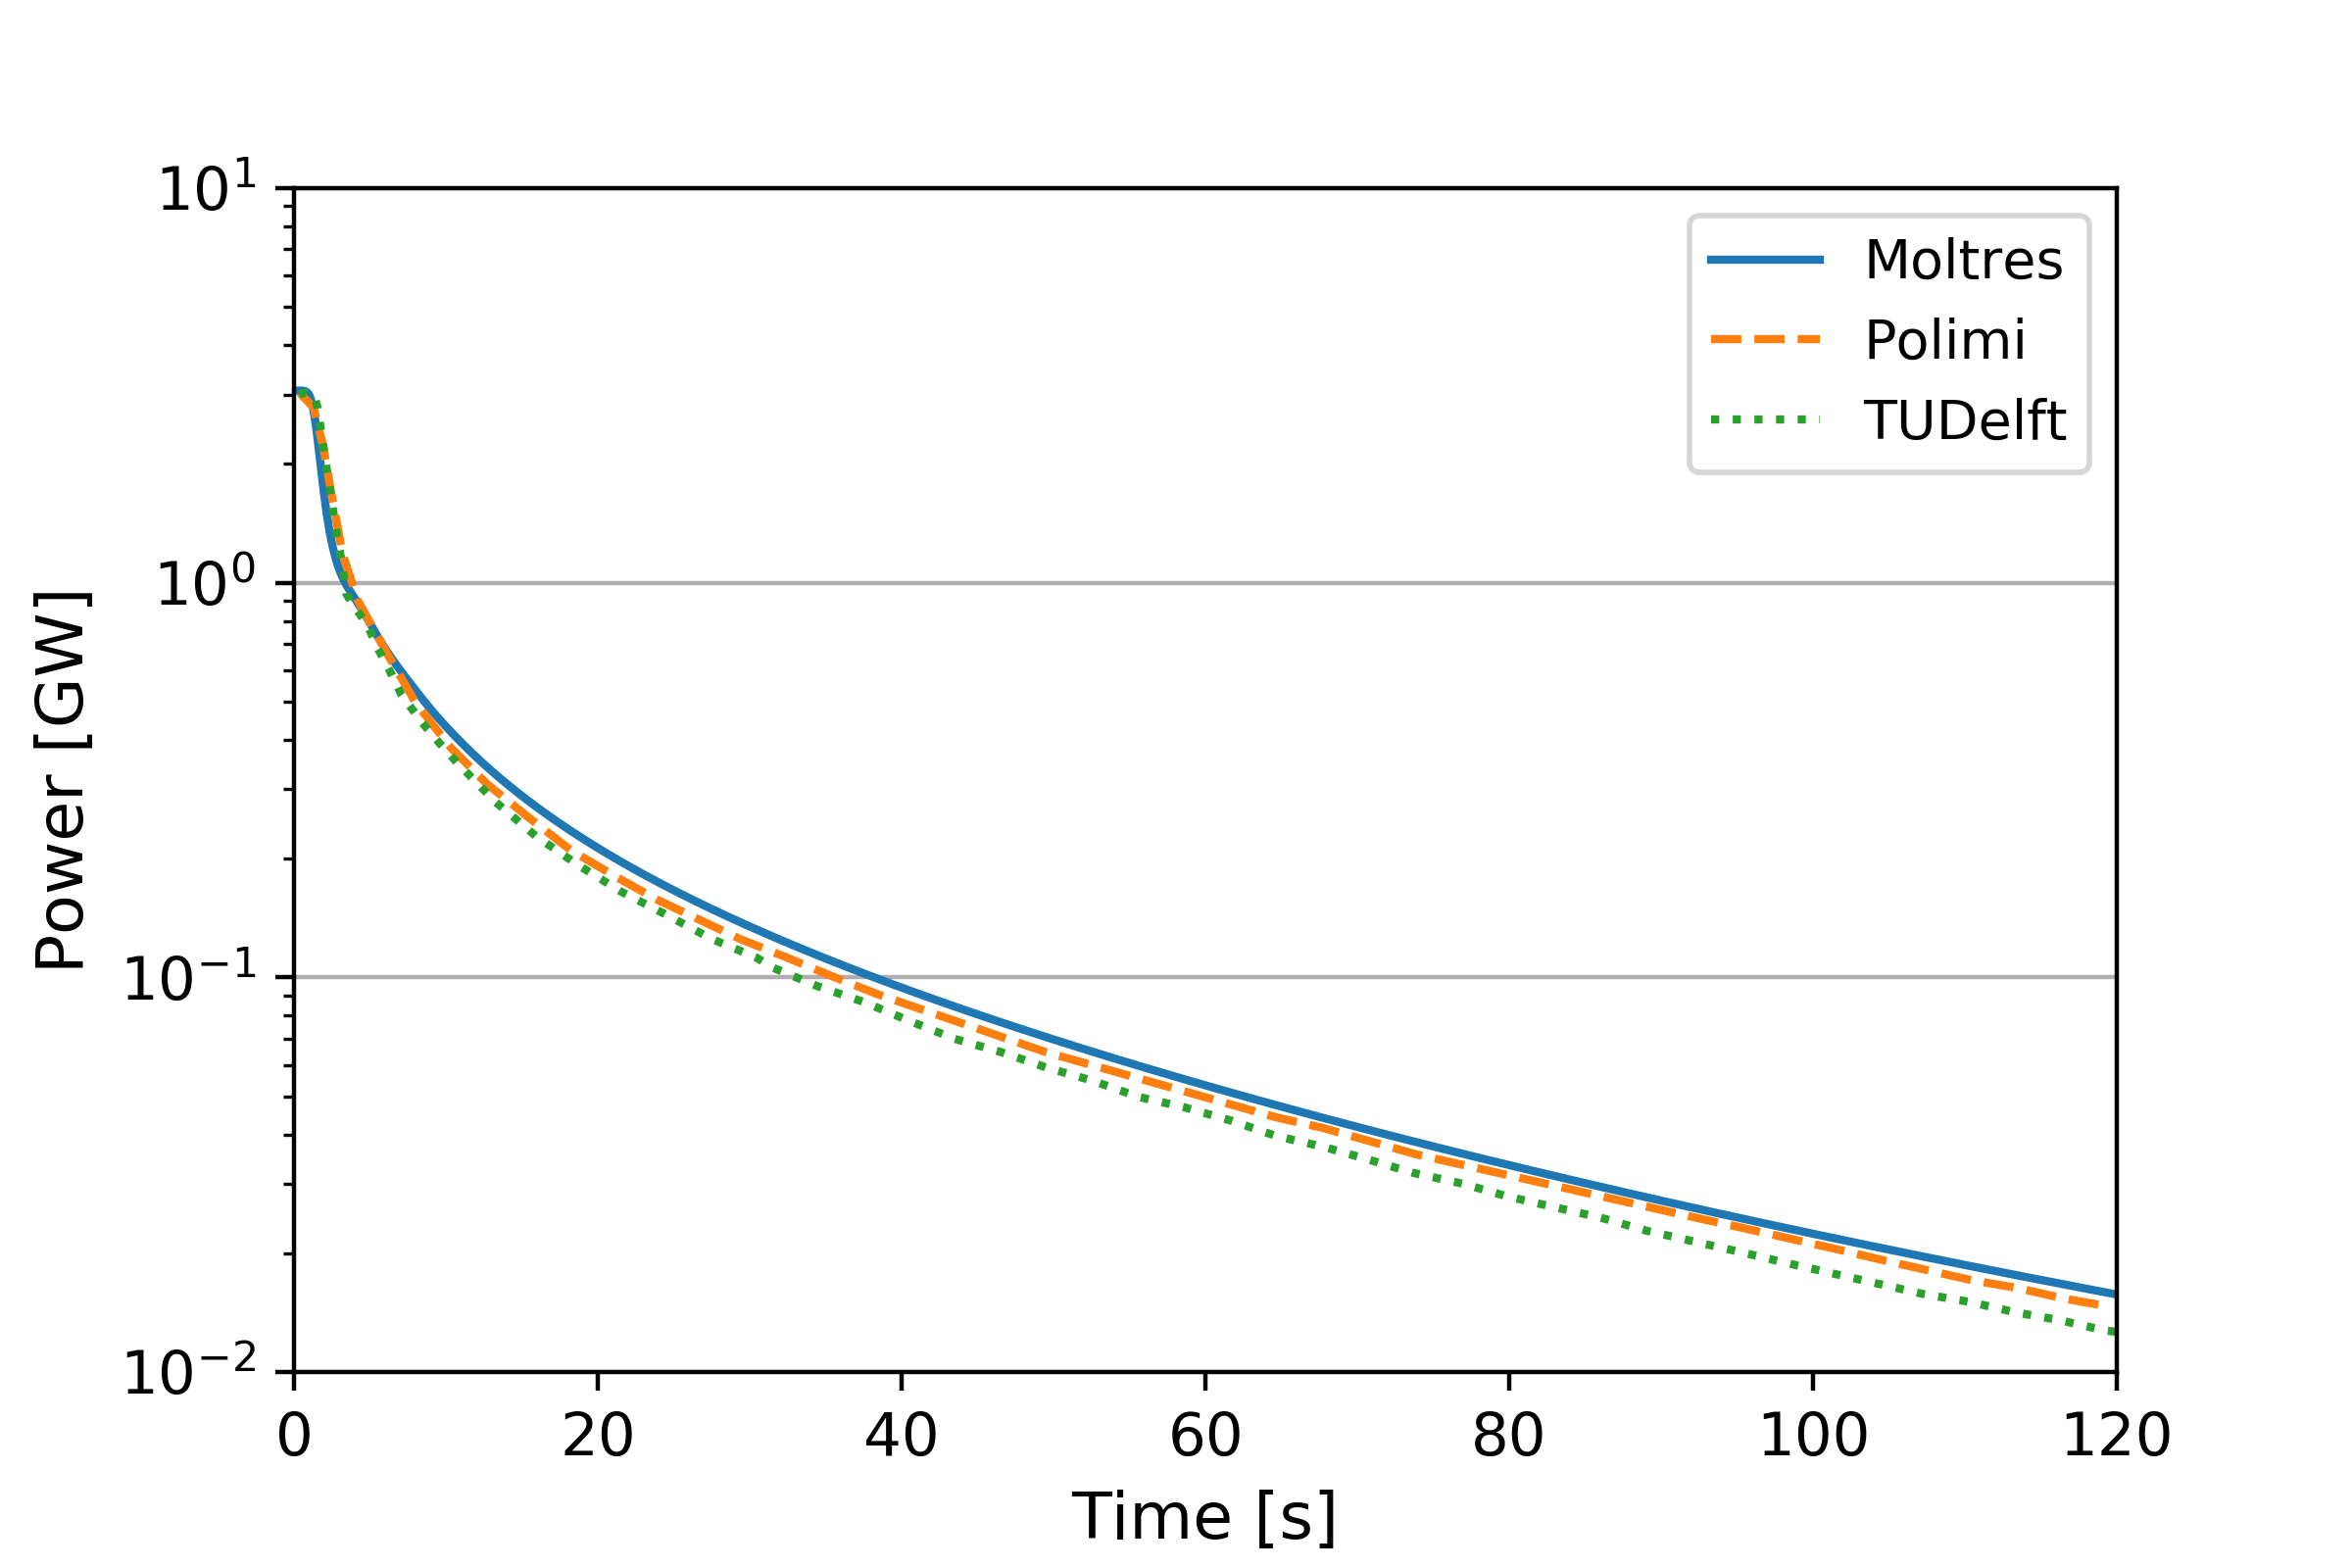
\includegraphics[width=.85\textwidth]{lohs-heat}
    \caption{Power output during
    an unprotected loss of heat sink transient in the Moltres, Polimi, and
    TUDelft models \cite{fiorina_modelling_2014}.}
    \label{fig:lohsheat}
    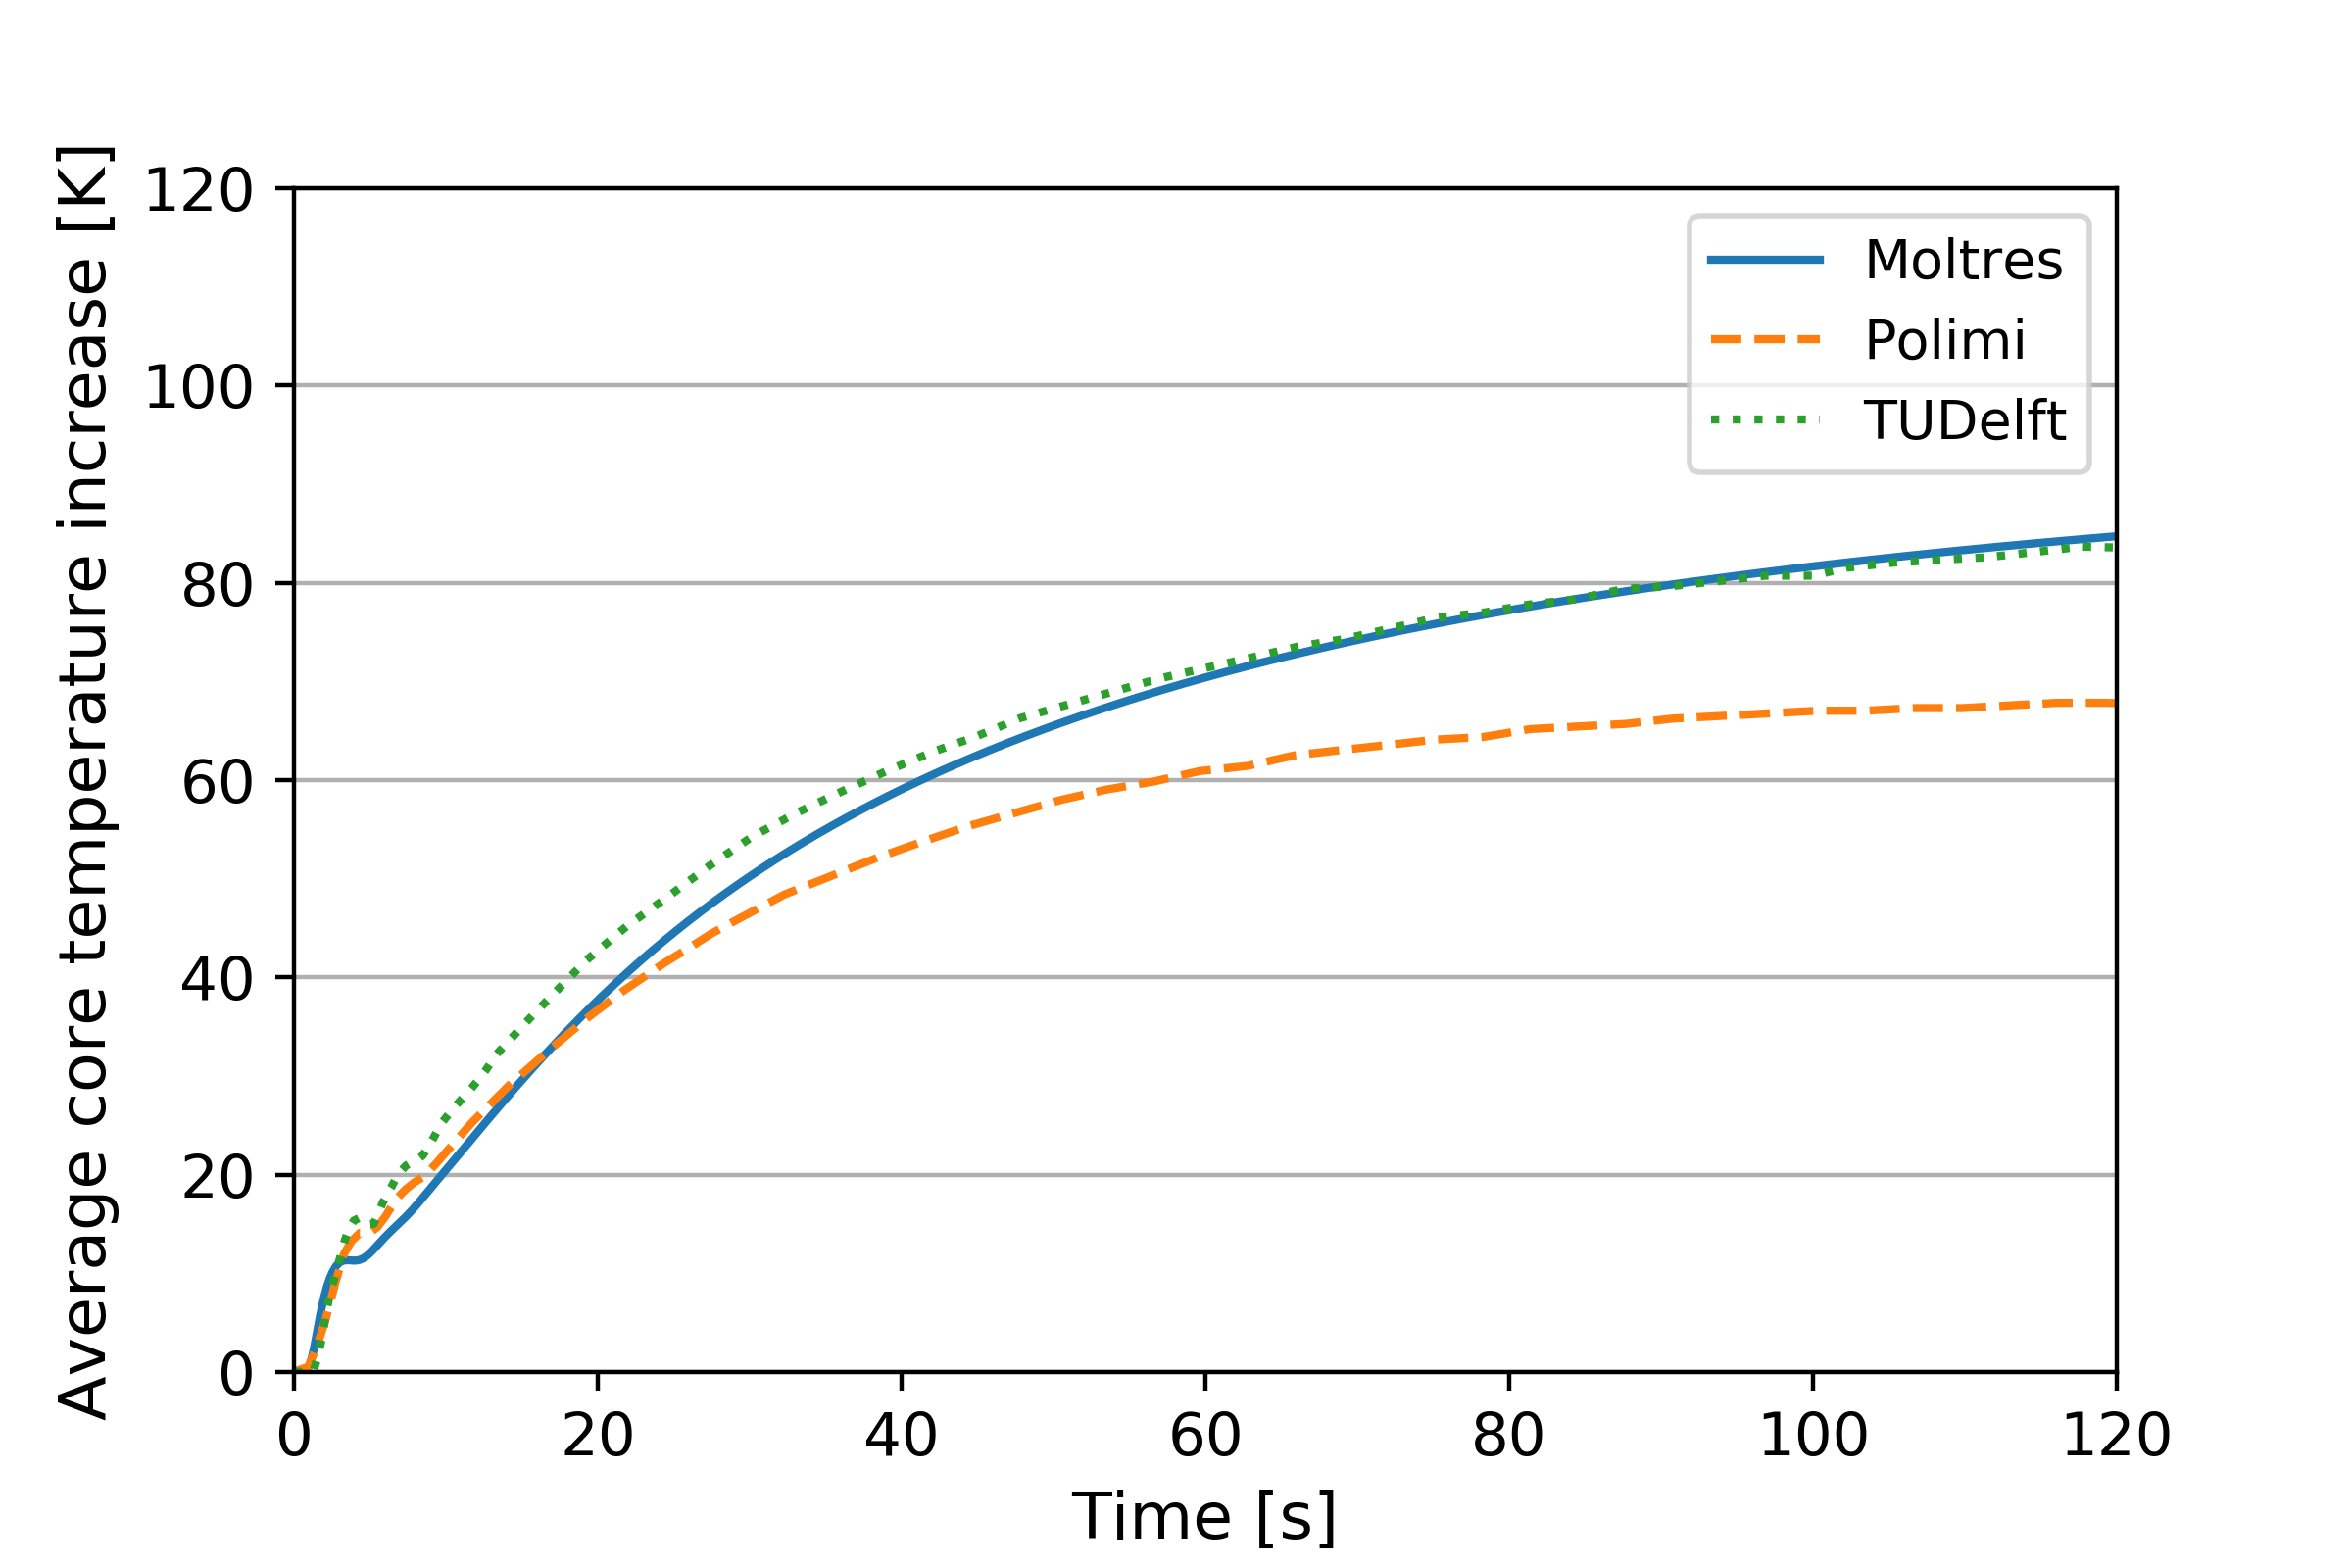
\includegraphics[width=.85\textwidth]{lohs-temp}
    \caption{Average core temperature increase during
    an unprotected loss of heat sink transient in the Moltres, Polimi, and
    TUDelft models \cite{fiorina_modelling_2014}.}
    \label{fig:lohstemp}
\end{figure}

\subsection{With Decay Heat}

\clearpage

\section{Unprotected Loss of Flow}

A loss of forced flow transient can occur in the event of a station
blackout; the pumps would cease operating due to the loss of AC electrical
power. Natural circulation resulting from temperature-dependent density
changes becomes the dominant driving force for salt flow in the primary loop.
While Fiorina et al. \cite{fiorina_modelling_2014} applied the Boussinesq
approximation for bouyancy-driven flow in their models, it is not directly
applicable to the \gls{MSFR} model in this thesis because we partitioned the
primary loop into two separate geometries and used Dirichlet boundary
conditions at the inlet to drive flow. Fiorina et al.'s Polimi and TUDelft
models featured complete exponential coast-downs of the pumps with a time
constant of 5 s. The resulting flow rate from natural circulation was
approximately 18 times smaller than the initial flow rate. Figure
\ref{fig:flowrate} shows that the actual flow rate decreased with a time
constant of 8 s. Thus, for the \gls{MSFR} model in Moltres, we imposed a
similar exponential decay term with a time constant of 8 s on the inflow
Dirichlet boundary condition:
%
\begin{align}
    \text{Flow rate, } v = 0.25862 + (4.5-0.25862) e^{-t/8} 
    \label{eq:flowrate}
\end{align}

\begin{figure}[htbp!]
    \centering
    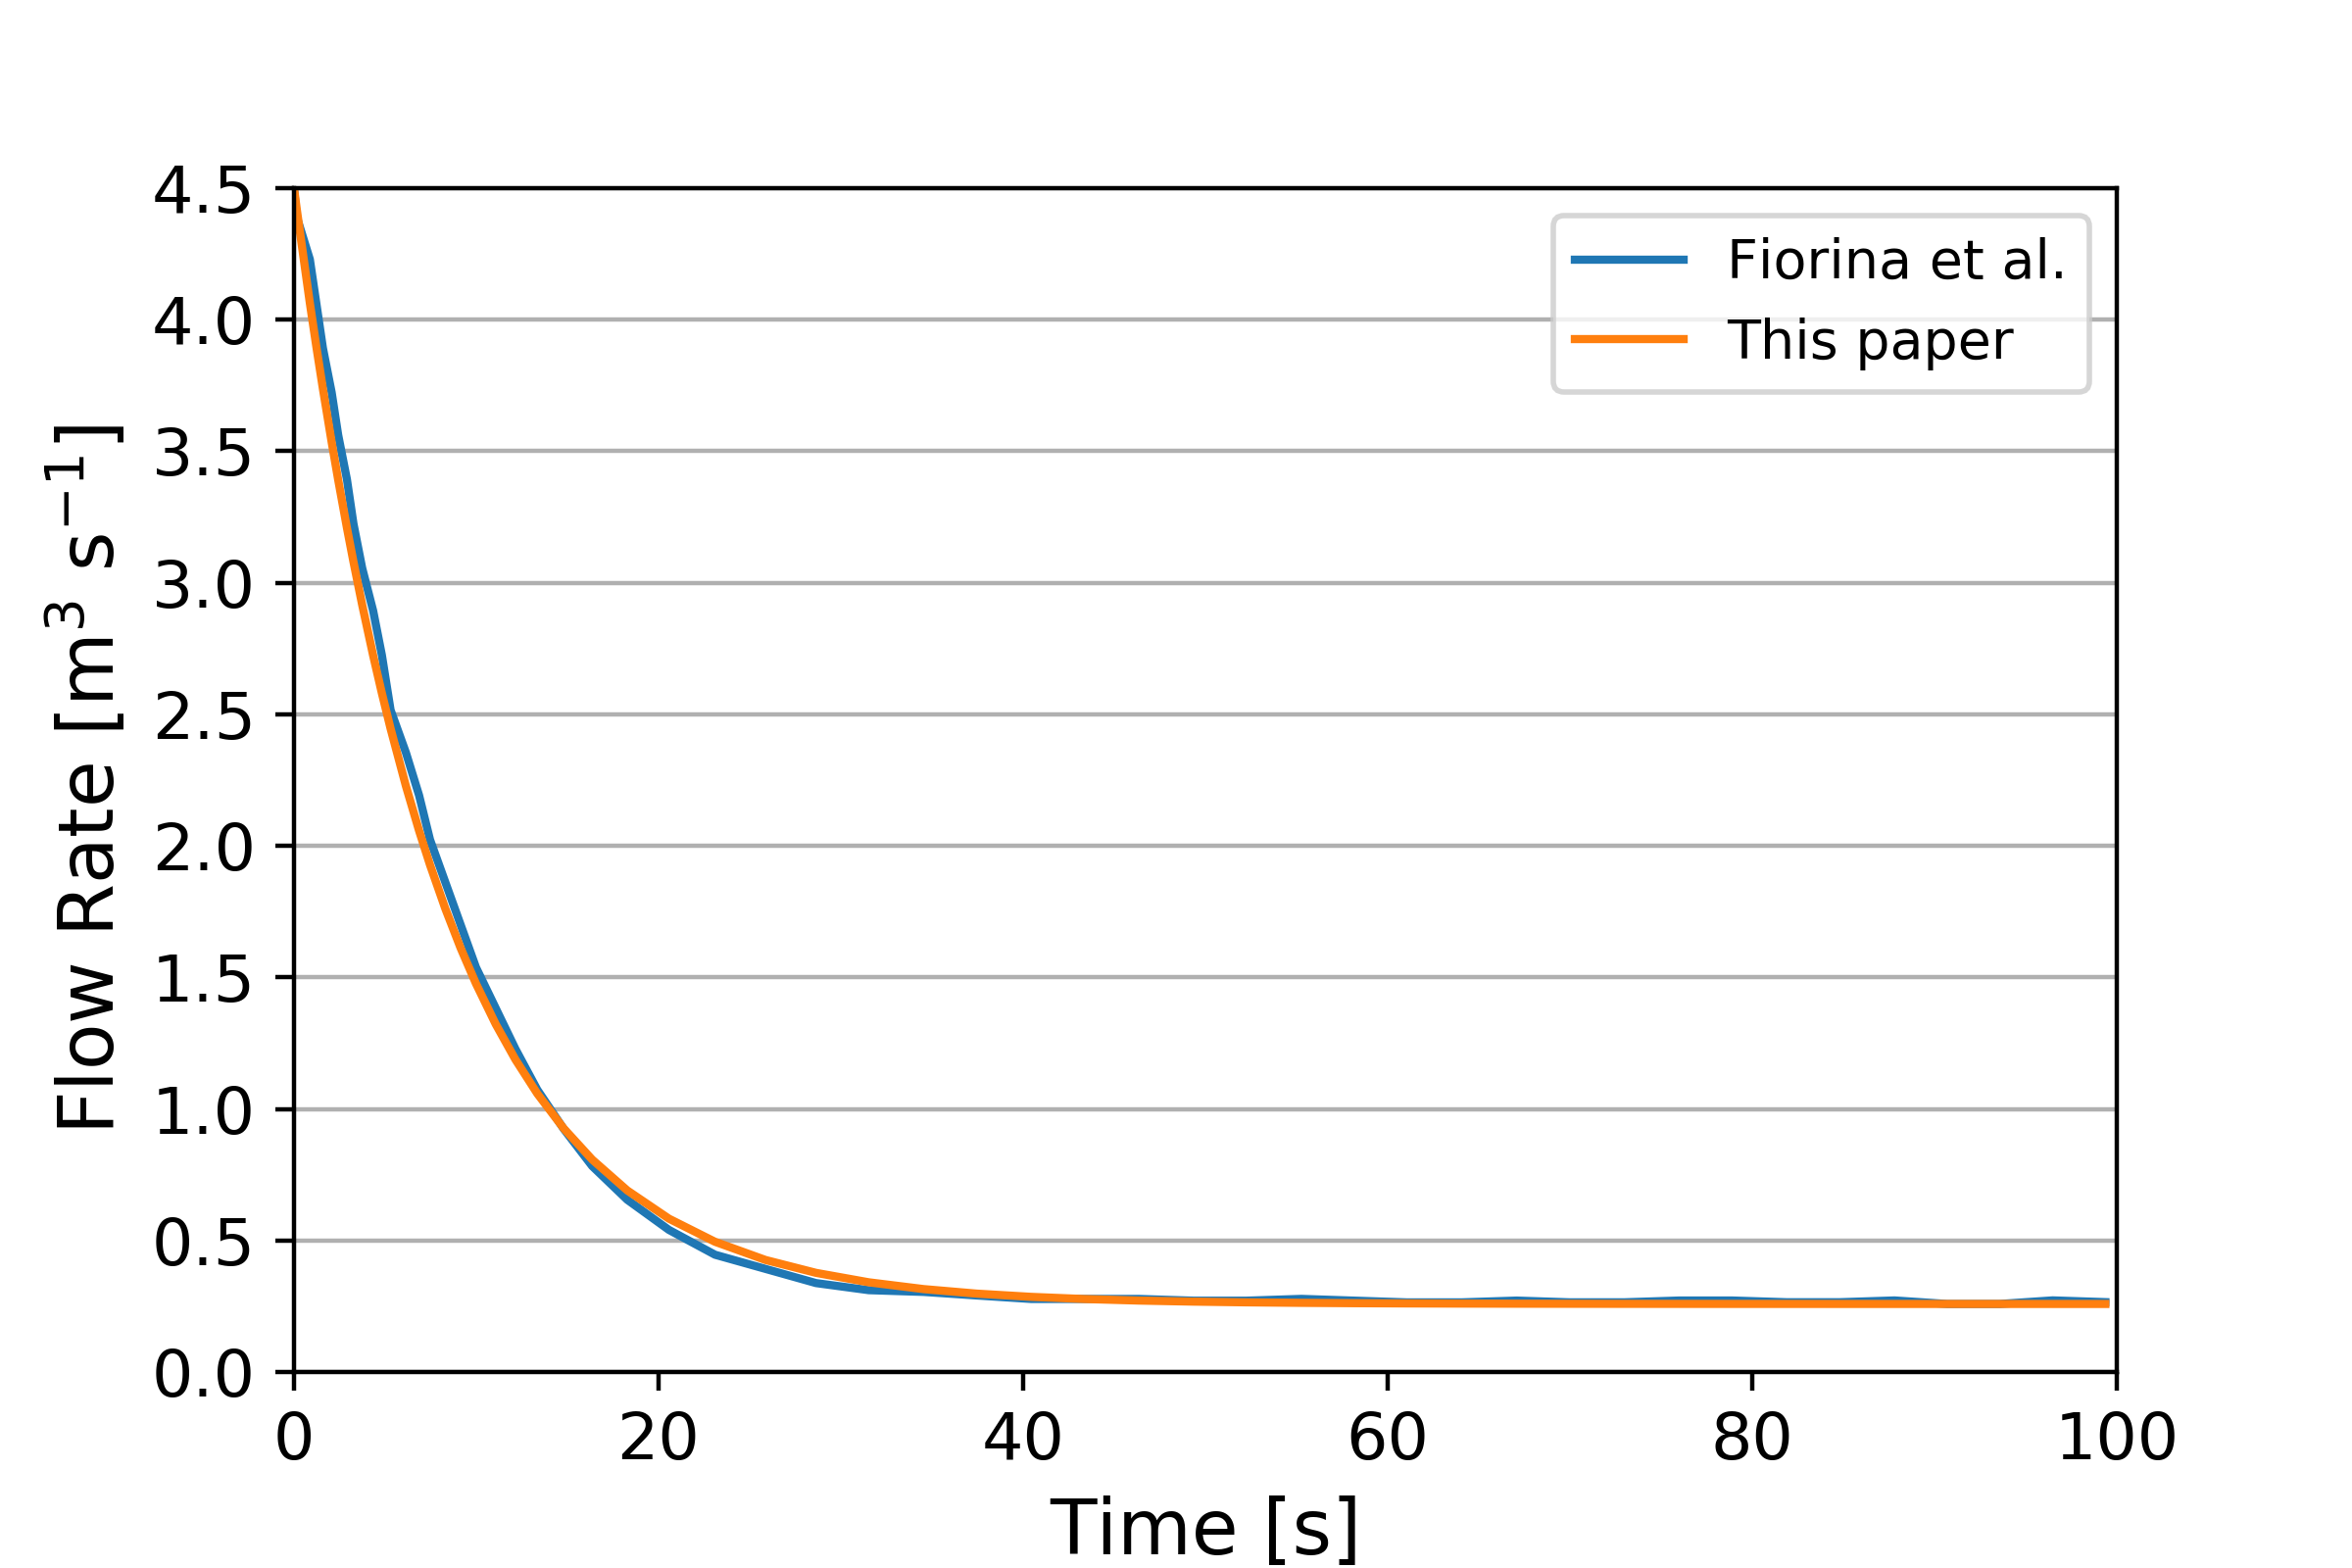
\includegraphics[width=.7\textwidth]{lof-flow-rate}
    \caption{The change in flow rate in the Polimi and TUDelft models and the
    imposed flow rate in Moltres.}
    \label{fig:flowrate}
\end{figure}

The reduced flow rate also decreases the heat transfer rate between the
primary and intermediate loop through the heat exchanger as the heat transfer
coefficient is dependent on the flow rate. This step was problematic because
the pointwise heat exchanger implementation in Moltres performs differently
compared to the heat exchangers that take up ``36\% of the out-of-core part''
in the Polimi and TUDelft models \cite{fiorina_modelling_2014}. Most of the
cooling happens in the top half of the heat exchanger where the temperature
differential between the primary and intermediate loops is the largest. In the
Polimi and TUDelft models, the overall heat transfer coefficient is the
``harmonic mean of the heat transfer coefficients on each side of the heat
exchanger''. For this loss of flow transient, the authors intended to focus on
the primary loop and assumed that only the pumps in the primary loop failed.
In addition to this, the authors applied the Dittus-Boelter correlation (cite
*) for
the relationship between the primary side heat transfer coefficient and the
flow rate. The Dittus-Boelter correlation for fluids being cooled is:
%
\begin{align}
    Nu &= 0.023 Re^{0.8} Pr^{0.3} \label{eq:db} \\
    \intertext{where}
    Nu &= \text{ Nusselt number,} \nonumber \\
    Re &= \text{ Reynolds number,} \nonumber \\
    Pr &= \text{ Prandtl number.} \nonumber
\end{align}

The only direct relation to flow velocity in the Dittus-Boelter correlation is
through the $Re$ term, which is directly proportional to flow velocity. This
gives the following relation between the heat transfer coefficient $h$ and
flow velocity $v$:
%
\begin{align}
    h \propto v^{0.8} \label{eq:hv}
\end{align}
%
However, this relation provided very different results in the unprotected loss
of flow and pump overspeed transients compared to the Polimi and TUDelft
models; it overpredicted the equilibrium power output in the
unprotected loss of flow transient and underpredicted the same parameter in
the unprotected pump overspeed transient. Upon further investigation, we found
that raising the power of $v$ from 0.8 to 1.1 brought the average core
temperatures closer to the results from the other models in both transients.
Therefore, we adopted the raised power in this study.

Another issue pertained to the turbulent viscosity $\mu_t$ as a function of
$v$. When we made a simple approximation of $\mu_t$ being directly
proportional to $v$, the results
differed significantly compared to the Polimi and TUDelft models (Appendix *).
This may have been due to buoyancy-driven flow contributing to turbulence; the
turbulent energy $k$ equation in the $k$-$\epsilon$ model has an explicit
source term from buoyancy effects (Cite *). Another point to note is the
Reynolds number does not change if $\mu$ and $v$ decrease in tandem. This
preserves the existence of the recirculation zone in the core and it is at
odds with the results from the Polimi and TUDelft models, which show that the
recirculation zones disappear during the loss of flow transient. We
circumvented this issue by letting higher fractions of $\mu_t$ be conserved
regardless of the final flow velocity. This measure allowed for laminar flow
to develop in the core and yielded results resembling those from the Polimi
and TUDelft models.

Figures * show


\section{Unprotected Pump Overspeed}

In the context of this thesis, pump overspeed refers to a sustained
increase in pump speed in the primary coolant loop. The increased flow rate
impacts reactor performance in several ways.
It affects the neutronics by reducing the in-core $\beta_eff$ as more of the
shorter-lived precursors will tend to flow out of the core before decaying.
This net loss of neutrons reduces the reactivity in the core, thereby causing
core temperatures to fall to counteract this change through temperature
reactivity feedback. The increased flow rate also enhances the heat transfer
coefficient on the primary loop side of the heat exchanger and enables the
reactor to operate at a higher power output. At the same time, the improved
mixing flattens the temperature distribution in the core.

We followed Fiorina et al.'s implementation \cite{fiorina_modelling_2014} by
ramping up the inlet velocity, $u$, by 50\% from the nominal value, $u_0$,
according to the following formula:

\begin{align}
    u(t) &= u_0 [1 + 0.5 (1 - e^{-t / \tau})] \\
    \intertext{where}
    \tau &= 5 \text{ s.} \nonumber
\end{align}
%
For this transient, we assumed that $\mu_t$ was directly proportional to $v$
because the buoyancy effects are negligible and the recirculation zones 
persist throughout the entire duration. Figures \ref{fig:poheat} and
\ref{fig:potemp} show the power output and average core temperature increase
during the unprotected pump overspeed transient in the Moltres, Polimi, and
TUDelft models.

Unlike in the loss of flow transient, the $\mu_t \propto v$ approximation
worked well in pump overspeed transient.

\begin{figure}[htbp!]
    \centering
    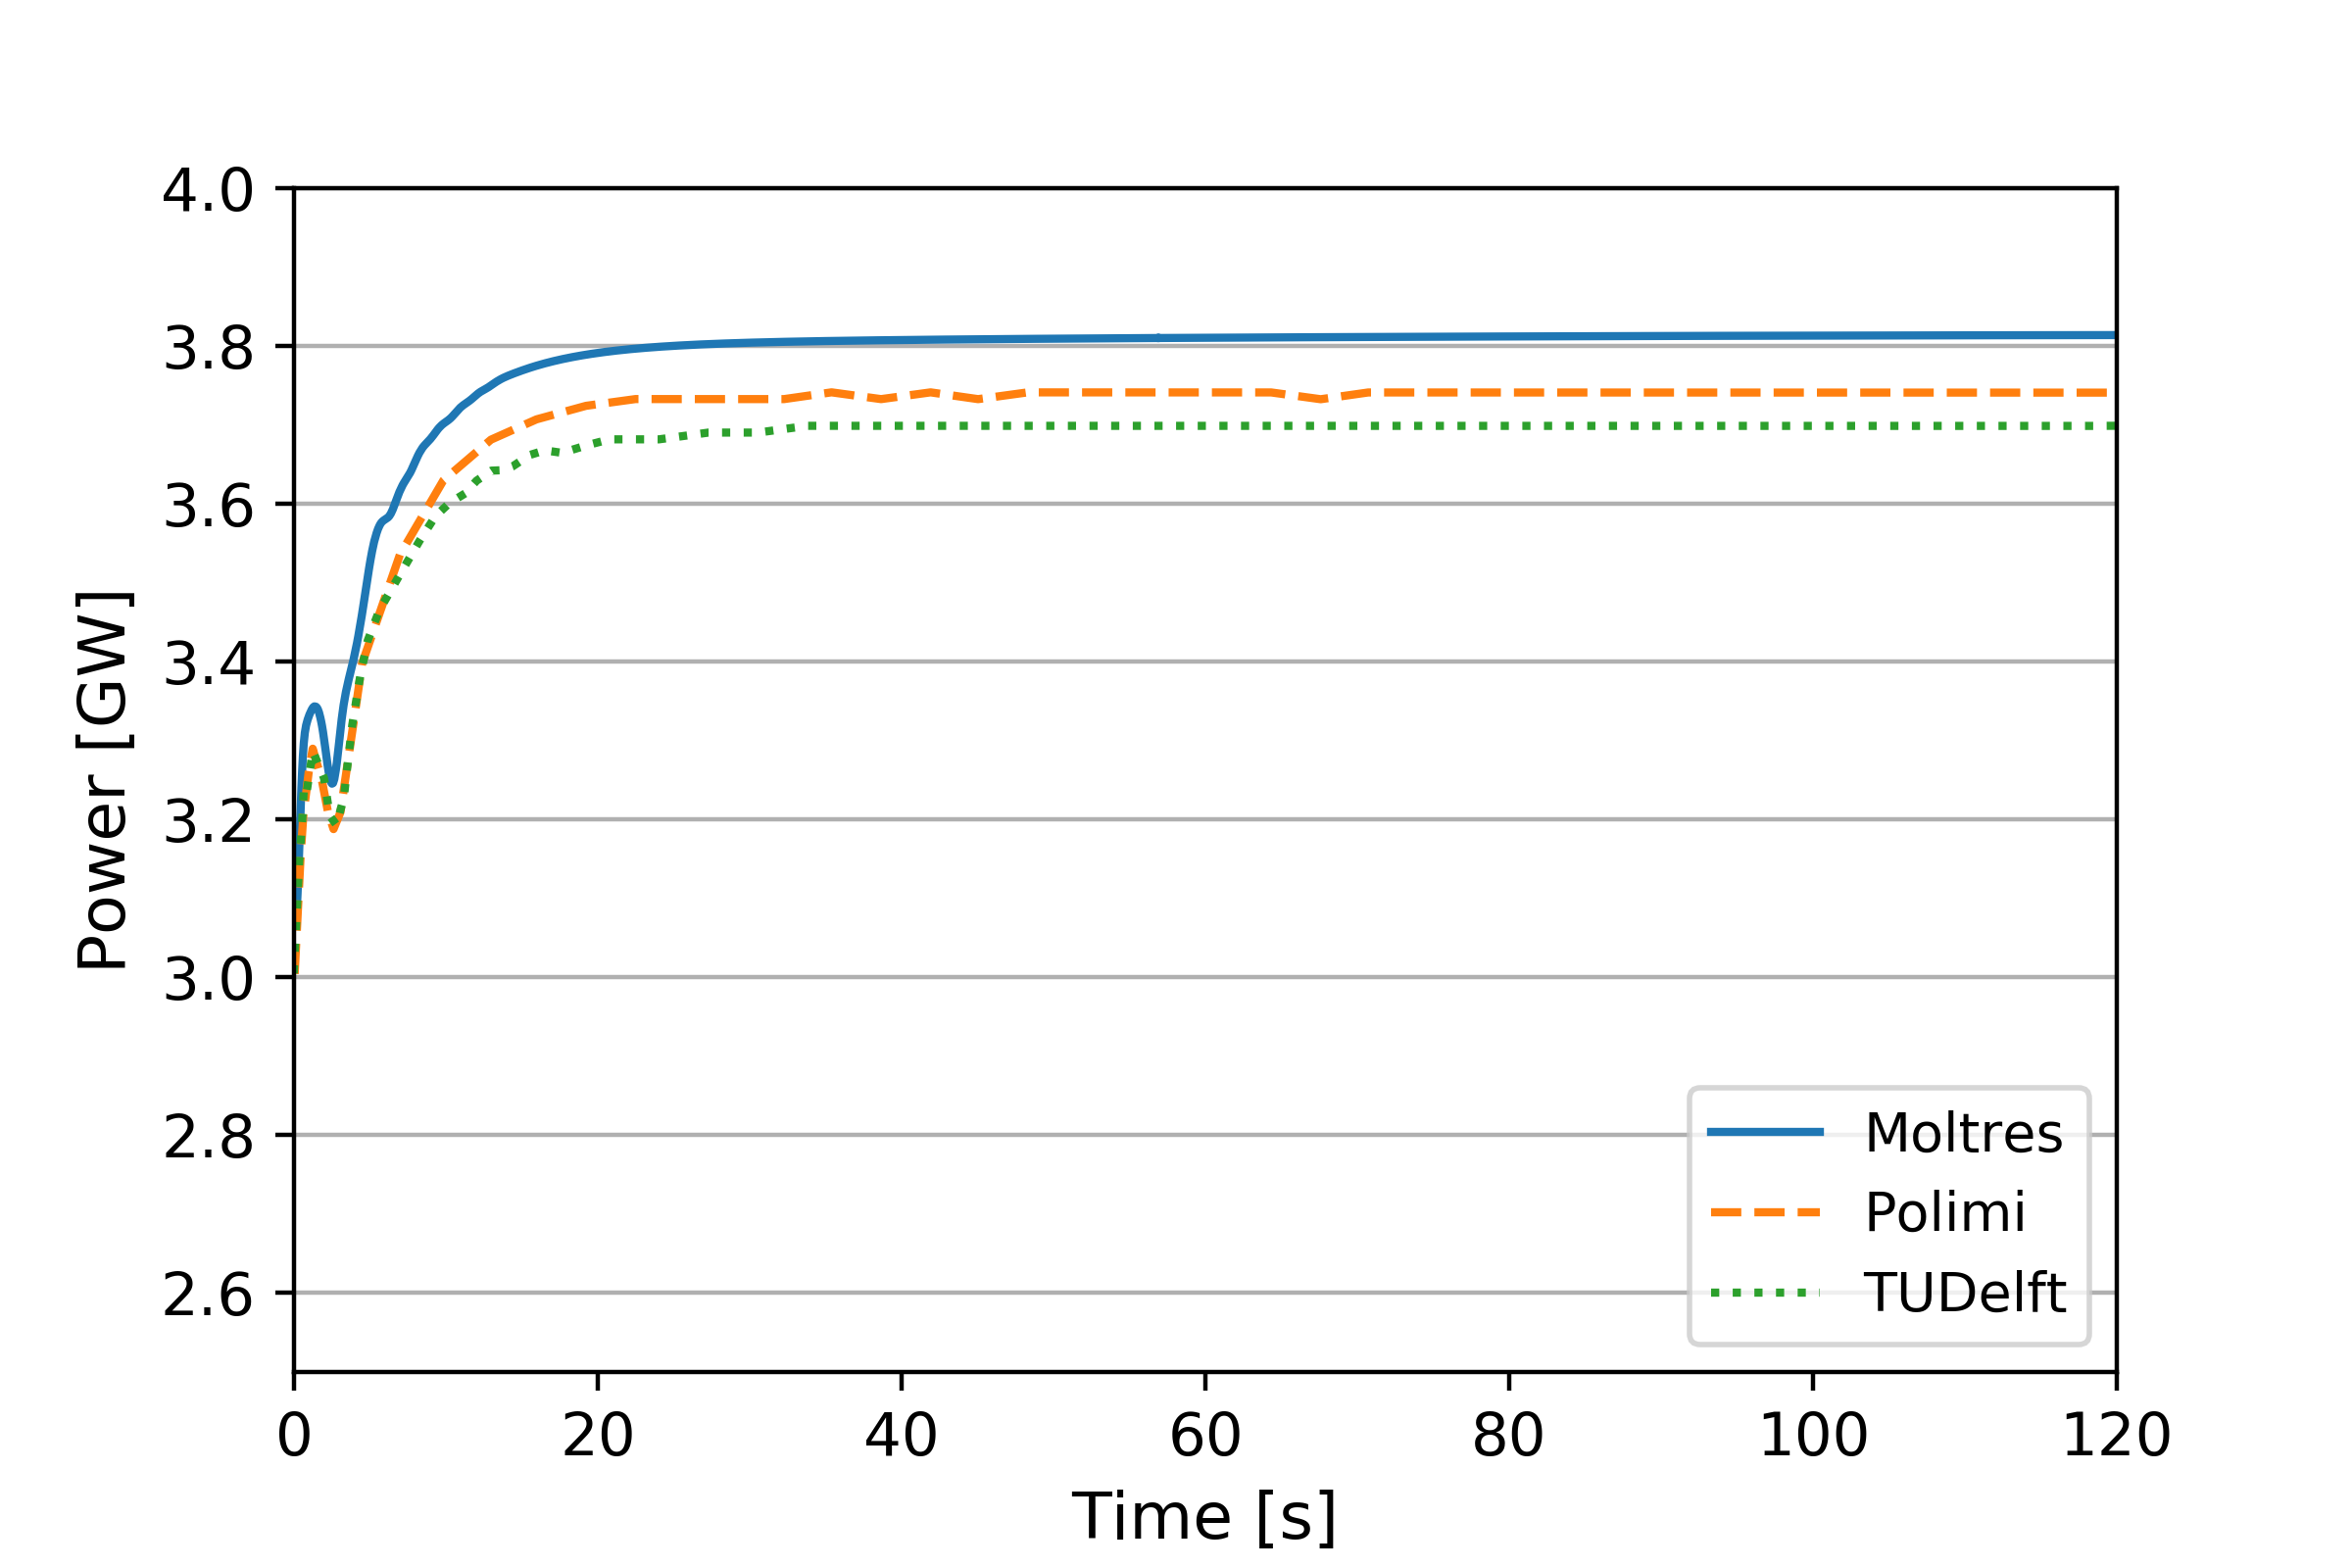
\includegraphics[width=.85\textwidth]{po-heat}
    \caption{Power output during
    an unprotected pump overspeed transient in the Moltres, Polimi, and
    TUDelft models \cite{fiorina_modelling_2014}.}
    \label{fig:poheat}
    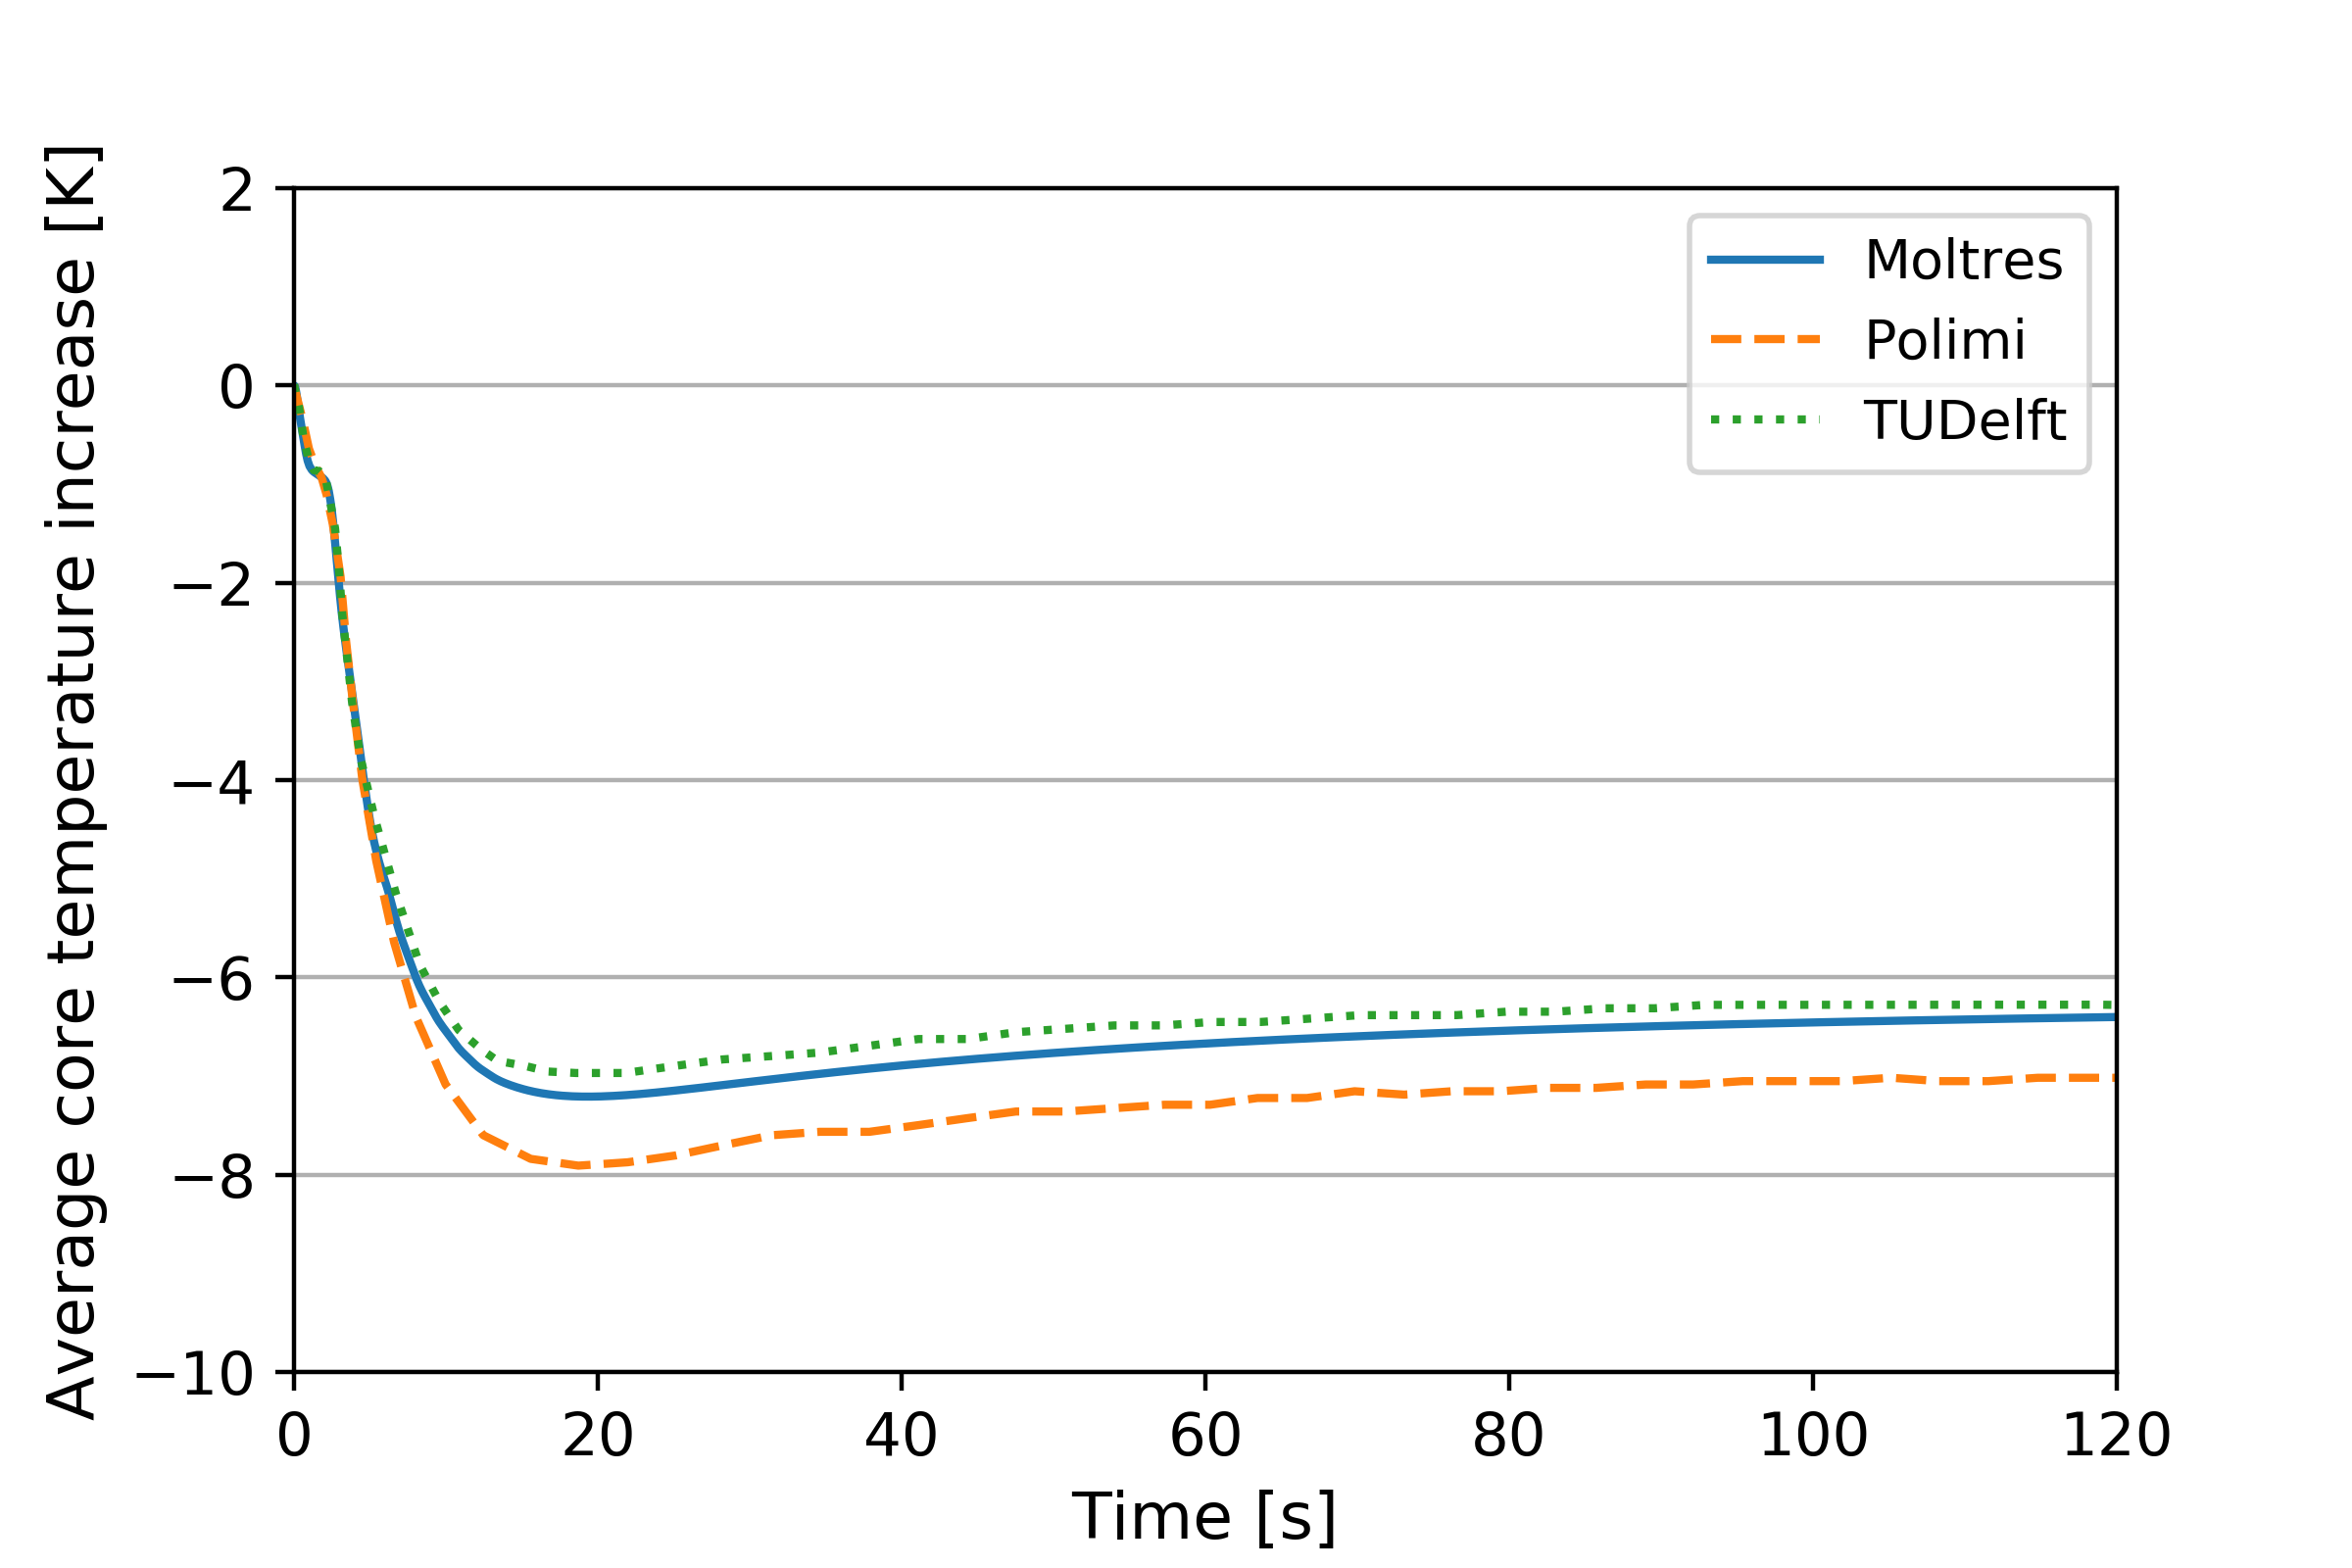
\includegraphics[width=.85\textwidth]{po-temp}
    \caption{Average core temperature increase during
    an unprotected pump overspeed transient in the Moltres, Polimi, and
    TUDelft models \cite{fiorina_modelling_2014}.}
    \label{fig:potemp}
\end{figure}
